
% !TEX TS-program = xelatex
% !TEX encoding = UTF-8 Unicode

\documentclass[aspectratio=169, 10pt]{beamer}

% --- Cấu hình Font & Tiếng Việt cho XeLaTeX ---
\usepackage{fontspec}
\usefonttheme{professionalfonts}
\setmainfont{Times New Roman}
\setsansfont{Times New Roman}
\setmonofont{Consolas}

% Hộp code — dùng trong frame [fragile]: \begin{codebox}\begin{verbatim}...\end{verbatim}\end{codebox}
\setbeamercolor{codebg}{bg=boxblue, fg=slate}
\newenvironment{codebox}{\begin{beamercolorbox}[sep=3pt, rounded=true]{codebg}\footnotesize\ttfamily}{\end{beamercolorbox}}

\usepackage{polyglossia}
\setdefaultlanguage{vietnamese}

\usepackage{amsmath, amssymb}
\usepackage{booktabs, colortbl, multirow, array}
\usepackage{tikz}
\usepackage{listings}
\lstdefinestyle{rnnpython}{
    language=Python,
    basicstyle=\ttfamily\scriptsize,
    keywordstyle=\color{blue},
    stringstyle=\color{warmorange},
    commentstyle=\color{emeraldgreen},
    showstringspaces=false,
    breaklines=true
}
\usetikzlibrary{shapes, arrows.meta, positioning, calc, matrix, fit, backgrounds, decorations.pathreplacing}
\usepackage{graphicx}

\usetheme{Madrid}
\usecolortheme{whale}
\setbeamertemplate{navigation symbols}{}

% Bảng màu thiết kế
\definecolor{mainnavy}{RGB}{26, 54, 93}
\definecolor{accentteal}{RGB}{13, 92, 117}
\definecolor{teal}{RGB}{13, 92, 117}
\definecolor{warmorange}{RGB}{217, 119, 6}
\definecolor{crimsonred}{RGB}{220, 38, 38}
\definecolor{emeraldgreen}{RGB}{5, 150, 105}
\definecolor{slate}{RGB}{51, 65, 85}
\definecolor{lightbg}{RGB}{248, 250, 252}
\definecolor{boxblue}{RGB}{239, 246, 255}
\definecolor{boxgreen}{RGB}{240, 253, 244}
\definecolor{boxorange}{RGB}{255, 251, 235}
\definecolor{boxred}{RGB}{254, 242, 242}

\setbeamercolor{structure}{fg=mainnavy}
\setbeamercolor{title}{bg=mainnavy, fg=white}
\setbeamercolor{frametitle}{bg=mainnavy, fg=white}
\setbeamercolor{block title}{bg=mainnavy, fg=white}
\setbeamercolor{block body}{bg=lightbg, fg=slate}
\setbeamercolor{block title example}{bg=accentteal, fg=white}
\setbeamercolor{block body example}{bg=lightbg, fg=slate}
\setbeamercolor{block title alerted}{bg=crimsonred, fg=white}
\setbeamercolor{block body alerted}{bg=boxred, fg=slate}

% Thanh chân trang chuẩn x / 24
\setbeamertemplate{footline}{%
  \leavevmode%
  \hbox{%
  \begin{beamercolorbox}[wd=.333333\paperwidth,ht=2.5ex,dp=1.1ex,center]{author in head/foot}%
    \usebeamerfont{author in head/foot}Deep Learning
  \end{beamercolorbox}%
  \begin{beamercolorbox}[wd=.333333\paperwidth,ht=2.5ex,dp=1.1ex,center]{title in head/foot}%
    \usebeamerfont{title in head/foot}Mạng Nơ-ron Hồi quy (RNN)
  \end{beamercolorbox}%
  \begin{beamercolorbox}[wd=.333333\paperwidth,ht=2.5ex,dp=1.1ex,right]{date in head/foot}%
    \usebeamerfont{date in head/foot}\insertframenumber{} / 38\hspace*{2.5ex}
  \end{beamercolorbox}}%
  \vskip0pt%
}

% Kiểu mũi tên TikZ
\tikzset{
  >=Stealth,
  flowarrow/.style={-{Stealth[length=2.2mm, width=1.5mm]}, thick, mainnavy},
  flowarrow_teal/.style={-{Stealth[length=2.2mm, width=1.5mm]}, thick, accentteal},
  flowarrow_red/.style={-{Stealth[length=2.2mm, width=1.5mm]}, thick, crimsonred},
  flowarrow_green/.style={-{Stealth[length=2.2mm, width=1.5mm]}, thick, emeraldgreen},
  flowarrow_orange/.style={-{Stealth[length=2.2mm, width=1.5mm]}, thick, warmorange},
  axisarrow/.style={-{Stealth[length=2.2mm, width=1.5mm]}, thick, mainnavy}
}

\title[Chuyên đề RNN]{MẠNG NƠ-RON HỒI QUY (RNN)}
\subtitle{Từ Hạn Chế của MLP \& 1D-CNN đến Nguyên Lý Xử Lý Dữ Liệu Chuỗi có Trạng Thái Ẩn}
\author{Nhóm thực hiện:\\Văn Thị Mai Linh \and Nguyễn Văn Minh Lực \and Giáp Minh Hiếu \and Nguyễn Nam Hải}
\institute{Chuyên đề Học Sâu (Deep Learning)}
\date{}

\begin{document}

% ---------------- SLIDE 1 ----------------
\begin{frame}[plain]
\titlepage
\vspace{-0.6cm}
\begin{center}
\textit{\footnotesize "Feedforward nhìn thế giới qua từng bức ảnh rời rạc;\\RNN thấu hiểu dữ liệu qua dòng chảy liên tục của thời gian."}
\end{center}
\end{frame}

% ---------------- SLIDE 2 ----------------
\begin{frame}{Bản chất Dữ liệu dạng Chuỗi (Sequential Data)}
\begin{block}{\textbf{Thứ tự xuất hiện quyết định hoàn toàn ngữ nghĩa của dữ liệu}}
\begin{itemize}
    \item \textbf{Đặc tính trật tự:} Mỗi điểm dữ liệu tại thời điểm \(t\) luôn mang mối tương quan mật thiết với các điểm quá khứ \(t-1, t-2, \dots\)
    \item \textbf{Hai dạng chính:} Dữ liệu token rời rạc (Text, DNA) và dữ liệu chuỗi số liên tục (Giá vàng, cổ phiếu, nhịp tim).
\end{itemize}
\end{block}

\vspace{0.3cm}
\begin{columns}[T]
\begin{column}{0.48\textwidth}
\begin{exampleblock}{\textbf{Chuỗi Rời rạc (NLP / Văn bản)}}
"Hà Nội không mưa" \(\neq\) "Mưa không Hà Nội"\\
\vspace{0.2cm}
\(\rightarrow\) \textit{Câu đầu có nghĩa rõ ràng, câu sau vô nghĩa hoặc biến đổi ngữ nghĩa.}
\end{exampleblock}
\end{column}
\begin{column}{0.48\textwidth}
\begin{alertblock}{\textbf{Chuỗi Liên tục (Time-Series)}}
Giá vàng: \([ 82.5 \rightarrow 83.1 \rightarrow 84.0 \rightarrow 85.2 ]\) (Tăng)\\
Giá vàng: \([ 85.2 \rightarrow 84.0 \rightarrow 83.1 \rightarrow 82.5 ]\) (Giảm)
\end{alertblock}
\end{column}
\end{columns}
\end{frame}

% ---------------- SLIDE 3 ----------------
\begin{frame}{Bài toán Dự đoán Phần tử Kế tiếp (Next Step Prediction)}
\textbf{Mục tiêu:} Cho chuỗi quan sát quá khứ \(X = (x_1, x_2, \dots, x_t)\), dự đoán giá trị tương lai \(x_{t+1}\).
\vspace{0.4cm}

\begin{block}{\textbf{Bài toán 1: Next Word Prediction (NLP)}}
Ngữ cảnh: \texttt{"We"} \(\rightarrow\) \texttt{"are"} \(\rightarrow\) \texttt{"learning"} \(\rightarrow\) \texttt{"AI"} \(\rightarrow\) \textbf{[ ? ]}\\
\(\rightarrow\) Target kỳ vọng: \textbf{"is"}
\end{block}

\begin{exampleblock}{\textbf{Bài toán 2: Dự báo Chuỗi thời gian (Time-Series)}}
Cửa sổ trượt (30 ngày lịch sử):\\
\([ P(t-29), P(t-28), \dots , P(t-1), P(t) ] \rightarrow \textbf{[ P(t+1) ]}\)\\
\(\rightarrow\) Dự báo biến động ngày 31.
\end{exampleblock}
\end{frame}

% ---------------- SLIDE 4 ----------------
\begin{frame}{Hai Pipeline Tiền xử lý Đặc trưng}
\textit{Dữ liệu thô không thể đưa trực tiếp vào mạng mà phải đi qua pipeline chuẩn hóa:}
\vspace{0.2cm}

\begin{columns}[T]
\begin{column}{0.48\textwidth}
\begin{block}{\textbf{Văn bản (Text Pipeline)}}
\footnotesize
\begin{enumerate}
    \item \textbf{Văn bản thô:} "giá vàng tăng"
    \item \textbf{Tokenizer:} ["giá", "vàng", "tăng"]
    \item \textbf{Vocab Index:} \([2, 3, 4]\)
    \item \textbf{Padding:} \([2, 3, 4, 0, 0]\)
    \item \textbf{Embedding:} Tensor \([\text{Batch}, \text{Seq\_Len}, d]\)
\end{enumerate}
\end{block}
\end{column}

\begin{column}{0.48\textwidth}
\begin{exampleblock}{\textbf{Chuỗi số (Time-Series Pipeline)}}
\small
\begin{enumerate}
    \item \textbf{File CSV thô:} Date, Price
    \item \textbf{Làm sạch \& Chia tập:} Train 70\%, Val 15\%, Test 15\%
    \item \textbf{Scaling:} log1p(Price) \(\rightarrow\) MinMax (chỉ fit trên Train)
    \item \textbf{Windowing:} Cửa sổ trượt 30 ngày
    \item \textbf{Đầu vào:} Tensor \([\text{N}, 30, 1]\)
\end{enumerate}
\end{exampleblock}
\end{column}
\end{columns}
\end{frame}

% ---------------- SLIDE 5 ----------------
\begin{frame}{Tiếp cận bằng MLP \& Cơ chế Ghép phẳng (Flatten)}
\textit{Mạng truyền thẳng (MLP) bắt buộc phải biến toàn bộ ngữ cảnh thành một vector phẳng duy nhất.}
\vspace{0.2cm}

\begin{center}
\begin{tikzpicture}[node distance=0.3cm, scale=0.8, every node/.style={scale=0.8}]
    \node[draw, rounded corners, fill=blue!10] (t1) {Token 1: \([ -0.18, 0.55, \dots ]\)};
    \node[draw, rounded corners, fill=blue!10, below=of t1] (t2) {Token 2: \([ 0.22, 1.32, \dots ]\)};
    \node[draw, rounded corners, fill=blue!10, below=of t2] (t3) {Token 3: \([ 0.43, -1.30, \dots ]\)};
    \node[draw, rounded corners, fill=blue!10, below=of t3] (t4) {Token 4: \([ 1.02, -1.90, \dots ]\)};
    \node[draw, rounded corners, fill=blue!10, below=of t4] (t5) {Token 5: \([ 1.78, -0.82, \dots ]\)};
    
    \node[draw, right=1.5cm of t3, fill=orange!20, minimum height=3cm, align=center] (concat) {Ép phẳng\\(Concatenate)\\ \(\rightarrow 1 \times 20\)};
    
    \draw[->, thick] (t1.east) -- (concat.west);
    \draw[->, thick] (t2.east) -- (concat.west);
    \draw[->, thick] (t3.east) -- (concat.west);
    \draw[->, thick] (t4.east) -- (concat.west);
    \draw[->, thick] (t5.east) -- (concat.west);
    
    \node[draw, right=1.5cm of concat, fill=green!20, align=center] (mlp) {Linear (20 \(\rightarrow\) 16)\\ ReLU \\ Linear (16 \(\rightarrow\) 8)};
    \draw[->, thick] (concat.east) -- (mlp.west);
    
    \node[draw, right=1.5cm of mlp, fill=red!20] (out) {Softmax \(\rightarrow\) "is"};
    \draw[->, thick] (mlp.east) -- (out.west);
\end{tikzpicture}
\end{center}
\end{frame}

% ---------------- SLIDE 6 ----------------
\begin{frame}[fragile]{Ví dụ: Tokenizer \& Vocabulary cho Next-Word Prediction}
\begin{columns}[T]
\begin{column}{0.57\textwidth}
\begin{block}{1. Code Python: tokenize, chuẩn hóa và tra ID}
\begin{lstlisting}[style=rnnpython]
text = "We are learning AI"
tokens = text.split()
tokens = [tok.lower() for tok in tokens]

vocab = {
    "[UNK]": 0, "[PAD]": 1, "ai": 2,
    "a": 3, "are": 4, "cs": 5,
    "is": 6, "learning": 7,
}
ids = [vocab.get(tok, vocab["[UNK]"]) for tok in tokens]
target = vocab["is"]
\end{lstlisting}
\end{block}

\begin{exampleblock}{2. Kết quả đầu ra}
\scriptsize
\texttt{tokens = ["we", "are", "learning", "ai"]}\\
\texttt{ids = [0, 4, 7, 2], target = 6}
\end{exampleblock}
\end{column}

\begin{column}{0.39\textwidth}
\centering
\scriptsize
\begin{tabular}{c l}
\toprule
\textbf{Index (ID)} & \textbf{Word / Token} \\
\midrule
0 & \texttt{[UNK]} (We) \\
1 & \texttt{[PAD]} \\
2 & \texttt{ai} \\
3 & \texttt{a} \\
4 & \texttt{are} \\
5 & \texttt{cs} \\
\rowcolor{yellow!25}
6 & \texttt{is} (Target) \\
7 & \texttt{learning} \\
\bottomrule
\end{tabular}

\vspace{0.12cm}
\textit{Tokenizer chỉ biến chuỗi thành token; vocabulary biến token thành ID.}
\end{column}
\end{columns}
\end{frame}

% ---------------- SLIDE 7 ----------------
\begin{frame}[fragile]{Padding \& Embedding: biến ID thành vector số}
\begin{columns}[T]
\begin{column}{0.48\textwidth}
\begin{block}{Code PyTorch: padding và embedding}
\begin{lstlisting}[style=rnnpython]
import torch
import torch.nn as nn
import torch.nn.functional as F

ids = torch.tensor([0, 4, 7, 2])
ids = F.pad(ids, (0, 1), value=1)
embedding = nn.Embedding(8, 4)
X = embedding(ids)
\end{lstlisting}
\end{block}

\begin{exampleblock}{Kết quả về kích thước}
\scriptsize
\texttt{ids = [0, 4, 7, 2, 1]}\\
\texttt{X.shape = torch.Size([5, 4])}
\end{exampleblock}
\end{column}

\begin{column}{0.48\textwidth}
\begin{block}{Ý nghĩa của từng bước}
\(L=5\) là cửa sổ đầu vào cố định; \texttt{[PAD]} chỉ được thêm để mọi mẫu có cùng chiều dài.

Nhãn cần dự đoán:
\[
y=6 \quad\Longleftrightarrow\quad \texttt{is}
\]
\end{block}

\begin{exampleblock}{Embedding lookup}
\scriptsize
Ma trận embedding \(E\in\mathbb{R}^{|V|\times d}=\mathbb{R}^{8\times4}\).

Mỗi ID được thay bằng một vector học được:
\[
\begin{bmatrix}
0\\4\\7\\2\\1
\end{bmatrix}
\;\longrightarrow\;
\begin{bmatrix}
e_0\\e_4\\e_7\\e_2\\e_1
\end{bmatrix}
\in\mathbb{R}^{5\times 4}
\]
\end{exampleblock}
\end{column}
\end{columns}
\end{frame}

% ---------------- SLIDE 8 ----------------
\begin{frame}[fragile]{MLP dự đoán từ tiếp theo: Forward Pass}
\begin{center}
\begin{tikzpicture}[node distance=0.35cm, every node/.style={font=\scriptsize}]
    \node[draw, rounded corners, fill=blue!10, align=center, text width=1.7cm, minimum height=1.0cm] (ids) {IDs\\\([0,4,7,2,1]\)};
    \node[draw, rounded corners, fill=violet!15, align=center, text width=2.1cm, minimum height=1.0cm, right=of ids] (embed) {Embedding\\\(5\times4\)};
    \node[draw, rounded corners, fill=orange!20, align=center, text width=2.0cm, minimum height=1.0cm, right=of embed] (flat) {Flatten\\\(1\times20\)};
    \node[draw, rounded corners, fill=green!20, align=center, text width=2.4cm, minimum height=1.0cm, right=of flat] (mlp) {Linear \(20\to16\)\\ReLU\\Linear \(16\to8\)};
    \node[draw, rounded corners, fill=red!15, align=center, text width=1.8cm, minimum height=1.0cm, right=of mlp] (softmax) {Softmax\\8 xác suất};

    \draw[->, thick] (ids) -- (embed);
    \draw[->, thick] (embed) -- (flat);
    \draw[->, thick] (flat) -- (mlp);
    \draw[->, thick] (mlp) -- (softmax);
\end{tikzpicture}
\end{center}

\vspace{0.08cm}
\begin{columns}[T]
\begin{column}{0.61\textwidth}
\begin{block}{Code PyTorch: Flatten và MLP}
\begin{lstlisting}[style=rnnpython]
import torch
import torch.nn as nn

X = torch.randn(5, 4)       # output cua Embedding
mlp = nn.Sequential(
    nn.Linear(5 * 4, 16), nn.ReLU(),
    nn.Linear(16, 8)
)
x = X.flatten().unsqueeze(0) # [1, 20]
logits = mlp(x)              # [1, 8]
\end{lstlisting}
\end{block}
\end{column}

\begin{column}{0.35\textwidth}
\begin{exampleblock}{Kích thước tensor}
\scriptsize
\texttt{X.shape = [5, 4]}\\
\texttt{x.shape = [1, 20]}\\
\texttt{logits.shape = [1, 8]}

\vspace{0.1cm}
Flatten biến 5 vector embedding thành một vector phẳng; MLP không còn thấy trạng thái theo thời gian.
\end{exampleblock}
\end{column}
\end{columns}
\end{frame}

% ---------------- SLIDE 9 ----------------
\begin{frame}[fragile]{Từ Softmax đến từ được dự đoán: Loss}
\begin{columns}[T]
\begin{column}{0.56\textwidth}
\begin{block}{Code PyTorch: Softmax và Cross-Entropy}
\begin{lstlisting}[style=rnnpython]
import torch
import torch.nn.functional as F
target_probs = torch.tensor([
    [.02, .04, .05, .02, .08, .06, .62, .11]])
logits = target_probs.log()
probs = F.softmax(logits, dim=-1)
y = torch.tensor([6])
loss = F.cross_entropy(logits, y)
print(probs.argmax(dim=-1).item()) # 6 = is
print(loss.item())                 # -log(0.62)
\end{lstlisting}
\end{block}

\begin{alertblock}{Ý nghĩa}
\scriptsize
\(p_i=\operatorname{softmax}(z)_i\), nhãn đúng là \(y=6\) (từ \texttt{is}):
\[
\mathcal{L}=-\log p_{6}
\]
Muốn loss nhỏ, mô hình phải đẩy xác suất của \texttt{is} lên cao.
\end{alertblock}
\end{column}

\begin{column}{0.38\textwidth}
\begin{exampleblock}{Ví dụ đầu ra}
\scriptsize
\begin{tabular}{l c}
\toprule
Token & Xác suất \\
\midrule
\texttt{ai} & 0.05 \\
\texttt{are} & 0.08 \\
\texttt{is} & \textbf{0.62} \\
\texttt{learning} & 0.11 \\
Các token khác & 0.14 \\
\bottomrule
\end{tabular}

\vspace{0.2cm}
\[
\hat{y}=\arg\max_i p_i=6
\]
\centering
\textbf{Dự đoán: ``is''}
\end{exampleblock}
\end{column}
\end{columns}
\end{frame}

% ---------------- SLIDE 10 ----------------
\begin{frame}{Từ giới hạn của MLP đến nhu cầu về RNN}
\vspace{-0.1cm}
\begin{center}
\begin{tikzpicture}[
    >=Stealth,
    mlpcard/.style={draw=crimsonred!65, fill=boxred, rounded corners=4pt,
        align=left, text width=4.55cm, minimum height=0.88cm, inner sep=6pt},
    rnncard/.style={draw=accentteal!75, fill=boxgreen, rounded corners=4pt,
        align=left, text width=4.55cm, minimum height=0.88cm, inner sep=6pt},
    arrow/.style={->, very thick, slate!80}
]
    \node[anchor=south, font=\small\bfseries, text=crimsonred] at (0,0.02) {MLP: ĐIỂM NGHẼN};
    \node[anchor=south, font=\small\bfseries, text=accentteal] at (8.5,0.02) {RNN: CƠ CHẾ ĐÁP ỨNG};

    \node[mlpcard] (m1) at (0,-0.95) {\textbf{1. Cửa sổ cố định \(L\)}\\[-2pt]
        \scriptsize Câu dài bị cắt; câu ngắn phải thêm padding.};
    \node[rnncard] (r1) at (8.5,-0.95) {\textbf{Trạng thái ẩn \(h_t\)}\\[-2pt]
        \scriptsize Đọc từng bước, giữ ngữ cảnh; nhận chuỗi dài ngắn khác nhau.};
    \draw[arrow] (m1.east) -- node[above, font=\scriptsize\bfseries, text=slate] {bộ nhớ linh hoạt} (r1.west);

    \node[mlpcard] (m2) at (0,-2.6) {\textbf{2. Flatten rời ngữ cảnh}\\[-2pt]
        \scriptsize Vị trí 1 và 5 là hai tọa độ độc lập; không có \(h_{t-1}\).};
    \node[rnncard] (r2) at (8.5,-2.6) {\textbf{Xử lý theo thứ tự thời gian}\\[-2pt]
        \scriptsize \(h_t=f(x_t,h_{t-1})\): mang theo ngữ cảnh quá khứ.};
    \draw[arrow] (m2.east) -- node[above, font=\scriptsize\bfseries, text=slate] {giữ thứ tự} (r2.west);

    \node[mlpcard, minimum height=1.6cm, inner xsep=6pt, inner ysep=3pt] (m3) at (0,-4.25) {\textbf{3. Tham số tăng theo \(L\)}\\[-2pt]
        \tiny Flatten: \(Ld\) đầu vào \(\to H\) neuron.\\[1pt]
        \(W\in\mathbb{R}^{H\times Ld}\): \(H(Ld)\) trọng số.\\[0pt]
        \(b\in\mathbb{R}^{H}\): \(H\) bias \(\Rightarrow H(Ld)+H\).\\[-1pt]
        \(64(30\cdot20)+64=38\,464\) tham số.};
    \node[rnncard] (r3) at (8.5,-4.25) {\textbf{Chia sẻ trọng số}\\[-2pt]
        \scriptsize Dùng lại cùng \(W,U,V\) ở mọi thời điểm \(t\).};
    \draw[arrow] (m3.east) -- node[above, font=\scriptsize\bfseries, text=slate] {chia sẻ} (r3.west);

    \node[draw=none, fill=mainnavy, rounded corners=5pt, text=white,
        align=center, text width=13.1cm, minimum height=0.82cm, inner sep=5pt]
        at (4.25,-5.8) {\large\bfseries RNN = BỘ NHỚ + THỨ TỰ + CHIA SẺ TRỌNG SỐ\\[-1pt]
        \normalsize \(x_t,\;h_{t-1}\;\longrightarrow\;h_t\;\longrightarrow\;y_t\)};
\end{tikzpicture}
\end{center}
\end{frame}
% ---------------- SLIDE 10 ----------------
\begin{frame}[fragile]{Ý tưởng Cốt lõi của RNN: Trạng thái Ẩn (\(h_t\))}
{\footnotesize\textbf{Trực giác:} Con người không bắt đầu tư duy lại từ đầu ở từng chữ, mà liên tục duy trì một dòng ý thức \textbf{nén dần thông tin quá khứ}.}

\vspace{0.03cm}
\begin{columns}[T]
% ---- Cột trái: sơ đồ đệ quy + ví dụ "Tôi đang học" ----
\begin{column}{0.46\textwidth}
\begin{center}
\begin{tikzpicture}[auto, thick, scale=0.74, every node/.style={scale=0.74}]
    \node (x1) [align=center] {\(t=1\) \\ "Tôi"};
    \node (x2) [right=1.0cm of x1, align=center] {\(t=2\) \\ "đang"};
    \node (x3) [right=1.0cm of x2, align=center] {\(t=3\) \\ "học"};

    \node (rnn1) [draw, fill=blue!10, rounded corners, below=0.7cm of x1, minimum width=1.2cm, minimum height=0.9cm] {RNN};
    \node (rnn2) [draw, fill=blue!10, rounded corners, below=0.7cm of x2, minimum width=1.2cm, minimum height=0.9cm] {RNN};
    \node (rnn3) [draw, fill=blue!10, rounded corners, below=0.7cm of x3, minimum width=1.2cm, minimum height=0.9cm] {RNN};

    \node (h0) [draw, fill=gray!20, rounded corners, below left=0.5cm and 0.25cm of rnn1] {\(h_0 = 0\)};

    \draw[flowarrow] (x1) -- (rnn1);
    \draw[flowarrow] (x2) -- (rnn2);
    \draw[flowarrow] (x3) -- (rnn3);

    \draw[flowarrow] (h0) -- (rnn1);
    \draw[flowarrow] (rnn1) -- (rnn2) node[midway, above] {\(h_1\)};
    \draw[flowarrow] (rnn2) -- (rnn3) node[midway, above] {\(h_2\)};
    \draw[flowarrow] (rnn3) -- ++(0.9,0) node[midway, above] {\(h_3\)};

    \begin{scope}[on background layer]
        \node[draw=crimsonred, dashed, rounded corners, fit=(rnn1) (rnn2) (rnn3), inner sep=4pt] (fitbox) {};
    \end{scope}
    \node[below=2pt of fitbox, text=crimsonred, font=\scriptsize\bfseries, align=center] {CÙNG MỘT Ô RNN\\(chung tham số \(\theta\))};
\end{tikzpicture}
\end{center}
\vspace{-0.05cm}
{\footnotesize
\textbf{\(h_t\) = "trí nhớ" nén toàn bộ quá khứ:}
\begin{itemize}\itemsep1pt
    \item \(h_1\): chỉ nhớ "Tôi"
    \item \(h_2\): nhớ "Tôi" + "đang"
    \item \(h_3\): nhớ trọn câu "Tôi đang học"
\end{itemize}}
\end{column}
% ---- Cột phải: lý thuyết đệ quy + code numpy ----
\begin{column}{0.52\textwidth}
\begin{exampleblock}{\textbf{Phương trình đệ quy của RNN}}
{\footnotesize Mỗi bước chỉ cần \textbf{trạng thái liền trước} \(h_{t-1}\) và \textbf{đầu vào hiện tại} \(x_t\): \(h_t = f_\theta\!\left(h_{t-1},\, x_t\right)\)}
\end{exampleblock}
\vspace{-0.06cm}
\begin{codebox}\begin{verbatim}
def rnn_cell(x_t, h_prev):
    a = W@x_t + U@h_prev + b_h  # tổng nhập
    return np.tanh(a)  # h_t - trí nhớ mới
h = np.zeros(d_h)  # h_0 = 0, chưa biết gì
for t in range(T):
    h = rnn_cell(x[t], h)  # cập nhật O(1)
\end{verbatim}\end{codebox}
\vspace{-0.02cm}
{\scriptsize
\begin{itemize}\itemsep1pt
    \item \textbf{Tóm tắt lịch sử vô hạn:} \(h_{t-1}\) đã chứa cả chuỗi quá khứ \(x_1, \ldots, x_{t-1}\), nên quá khứ dài bao nhiêu cũng được nén vào vector \textbf{cố định \(d_h\) chiều}.
    \item \textbf{Cập nhật từng bước \(O(1)\):} mỗi token đến chỉ cần \textbf{một} phép cập nhật; xử lý kiểu streaming, không phải lưu toàn chuỗi trong bộ nhớ.
    \item \textbf{Khác MLP cửa sổ trượt:} MLP phải thấy đủ \(L\) phần tử trong cửa sổ; RNN duy trì "tóm tắt động" \(h_t\) \textbf{không phụ thuộc độ dài} chuỗi.
\end{itemize}}
\end{column}
\end{columns}
\end{frame}

% ---------------- SLIDE 11 ----------------
\begin{frame}[fragile]{Công thức Toán học -- Quá trình Forward}
\footnotesize
{\footnotesize Ba phương trình forward tại bước \(t\), với \(x_t \in \mathbb{R}^{d_x}\) (đầu vào), \(h_t \in \mathbb{R}^{d_h}\) (trạng thái ẩn), \(\hat{y}_t \in \mathbb{R}^{d_y}\) (dự đoán):}
\vspace{-0.2cm}
\setlength{\abovedisplayskip}{0pt}
\setlength{\belowdisplayskip}{0pt}
\setlength{\jot}{1pt}
\begin{align*}
    a_t &= \mathbf{W} x_t + \mathbf{U} h_{t-1} + b_h
    && \text{\footnotesize tổng nhập: ghép tin mới với trí nhớ cũ} \\
    h_t &= \tanh(a_t)
    && \text{\footnotesize trạng thái ẩn mới, truyền sang bước \(t+1\)} \\
    \hat{y}_t &= \mathbf{V} h_t + b_y
    && \text{\footnotesize đọc bộ nhớ \(h_t\) để đưa ra dự đoán}
\end{align*}
\vspace{-0.25cm}
\begin{columns}[T]
\begin{column}{0.54\textwidth}
\centering
\footnotesize
\setlength{\tabcolsep}{4pt}
\begin{tabular}{@{}clll@{}}
\toprule
\textbf{Tham số} & \textbf{Kích thước} & \textbf{Kết nối} & \textbf{Vai trò} \\
\midrule
\(\mathbf{W}\) & \(d_h \times d_x\) & Vào \(\rightarrow\) Ẩn & Đọc tin mới \(x_t\) \\
\addlinespace[1pt]
\(\mathbf{U}\) & \(d_h \times d_h\) & Ẩn \(\rightarrow\) Ẩn & Giữ trí nhớ \(h_{t-1}\) \\
\addlinespace[1pt]
\(\mathbf{V}\) & \(d_y \times d_h\) & Ẩn \(\rightarrow\) Ra & Đọc ra kết quả \\
\addlinespace[1pt]
\(b_h,\ b_y\) & \(d_h,\ d_y\) & Bias & Dịch ngưỡng \\
\bottomrule
\end{tabular}
\end{column}
\begin{column}{0.43\textwidth}
\centering
\begin{tikzpicture}[thick, scale=0.70, every node/.style={scale=0.70}]
    \node (hprev) [draw, rounded corners, fill=gray!20, minimum width=1.4cm] {\(h_{t-1}\)};
    \node (xt) [draw, rounded corners, fill=green!20, minimum width=1.4cm, below=0.45cm of hprev] {\(x_t\)};
    \node (ht) [draw, rounded corners, fill=blue!20, minimum width=1.6cm, right=1.2cm of hprev, yshift=-0.55cm] {\(h_t\)};
    \node (yt) [draw, rounded corners, fill=orange!20, minimum width=1.5cm, right=1.0cm of ht] {\(\hat{y}_t\)};
    \draw[flowarrow] (hprev.east) -- (ht.north west) node[pos=0.45, above left] {\(\mathbf{U}\)};
    \draw[flowarrow_green] (xt.east) -- (ht.south west) node[pos=0.45, below left] {\(\mathbf{W}\)};
    \draw[flowarrow_orange] (ht.east) -- (yt.west) node[midway, above] {\(\mathbf{V}\)};
    \node[below=0.03cm of hprev, font=\scriptsize, text=slate] {trí nhớ cũ};
    \node[below=0.03cm of xt, font=\scriptsize, text=slate] {tin mới};
    \node[below=0.03cm of ht, font=\scriptsize, text=slate] {bộ nhớ mới};
    \node[below=0.03cm of yt, font=\scriptsize, text=slate] {dự đoán};
\end{tikzpicture}
\end{column}
\end{columns}
\vspace{-0.1cm}
\begin{codebox}\begin{verbatim}
a_t = W @ x_t + U @ h_prev + b_h   # (1) tổng nhập
h_t = np.tanh(a_t)                 # (2) trạng thái ẩn
y_hat = V @ h_t + b_y              # (3) dự đoán
\end{verbatim}\end{codebox}
\vspace{-0.1cm}
\footnotesize
\begin{itemize}\itemsep-1pt
    \item \textbf{Vì sao hàm \(\tanh\)?} Tâm \(0\), chặn \((-1,1)\) nên chuẩn của \(h_t\) ổn định qua các bước, đạo hàm \(1-\tanh^2(a_t)\) gọn; \textit{sigmoid} lệch dương (trung bình \(1/2\)), đạo hàm \(\leq 0.25\) làm gradient tắt nhanh; \textit{ReLU} không chặn trên, trạng thái cộng dồn dễ bùng nổ.
    \item \textbf{Tên PyTorch tương ứng:} \(\mathbf{W}\) = \texttt{weight\_ih\_l0}, \(\mathbf{U}\) = \texttt{weight\_hh\_l0} (Keras: \texttt{kernel}, \texttt{recurrent\_kernel}); mất mát tổng theo thời gian \(L = \sum_{t=1}^{T} \ell(\hat{y}_t, y_t)\) (MSE cho hồi quy).
\end{itemize}
\end{frame}

% ---------------- SLIDE 12 ----------------
\begin{frame}[fragile]{Ví dụ Tính Toán Forward Từng Bước (số cụ thể)}

% Thiết lập số: W, U, V, x1, h0 chuyển vào hộp code (cột phải); header chỉ còn kích thước + bias
\begin{center}
\footnotesize
$d_x = 2$, $\;d_h = 2$, $\;d_y = 1$;\quad $\mathbf{b}_h = \mathbf{0}$,\; $b_y = 0.1$
\end{center}

\vspace{0.05cm}
\begin{columns}[T]

\begin{column}{0.52\textwidth}
\scriptsize
\setlength{\tabcolsep}{2.5pt}
\renewcommand{\arraystretch}{1.1}
\resizebox{\linewidth}{!}{%
\begin{tabular}{@{}clll@{}}
\toprule
\textbf{Bước} & \textbf{Phép tính} & \textbf{Ý nghĩa} & \textbf{Kết quả ($t = 1$)} \\
\midrule
1 & $W \cdot \mathbf{x}_1$ & Đọc tin mới & $(+0.500,\; -0.100)$ \\
2 & $U \cdot \mathbf{h}_0$ & \shortstack{Chưa có ký ức\\(trang trắng)} & $(+0.000,\; +0.000)$ \\
\rowcolor{lightbg}
3 & $\mathbf{h}_1 = \tanh(W \cdot \mathbf{x}_1 + U \cdot \mathbf{h}_0 + \mathbf{b}_h)$ & \shortstack{Ký ức mới\\(vector)} & \textcolor{accentteal}{$(+0.462,\; -0.100)$} \\
4 & $\hat{y}_1 = V \cdot \mathbf{h}_1 + b_y$ & Đầu ra (số) & \textcolor{warmorange}{$+0.662$} \\
\bottomrule
\end{tabular}}

\vspace{0.08cm}
\footnotesize
\textbf{Bước $t = 2$: lặp nguyên hệ thống.} Thay $\mathbf{x}_2 = (0,\, 1)$, lấy $\mathbf{h}_1$ vừa tính làm \emph{trí nhớ cũ} (lúc này $U \cdot \mathbf{h}_1 \neq \mathbf{0}$: thành phần hồi quy xuất hiện lần đầu); bộ trọng số $(W, U, V)$ giữ nguyên tuyệt đối, chạy dần đến $t = T$.

\vspace{0.08cm}
\begin{center}
\textbf{Shape flow:}\; $\mathbf{x} \in \mathbb{R}^{T \times d_x} \;\longrightarrow\; \mathbf{h} \in \mathbb{R}^{T \times d_h} \;\longrightarrow\; \hat{\mathbf{y}} \in \mathbb{R}^{T \times d_y}$
\end{center}
\end{column}

\begin{column}{0.45\textwidth}
\begin{codebox}\scriptsize\begin{verbatim}
W = np.array([[0.5, 0.2],
              [-0.1, 0.4]])
U = np.array([[0.3, 0.0],
              [0.2, 0.5]])
V = np.array([[1.0, -1.0]])
x1 = np.array([1.0, 0.0]); h0 = np.zeros(2)
h1 = np.tanh(W @ x1 + U @ h0 + 0)
#  -> [0.462, -0.100]  (bước 3)
y1 = (V @ h1 + 0.1)[0]
#  -> 0.662           (bước 4)
\end{verbatim}\end{codebox}

\vspace{0.06cm}
{\scriptsize \textcolor{slate}{\textit{Ghi chú: PyTorch \texttt{nn.RNN(2,\,2)} + \texttt{nn.Linear(2,\,1)} nạp đúng $W$, $U$, $V$, đặt 2 bias của \texttt{nn.RNN} về 0 và bias \texttt{Linear} $= 0.1$ thì chạy đúng ví dụ (sai số $< 10^{-6}$).}}}
\end{column}
\end{columns}

\end{frame}

% ---------------- SLIDE 13 ----------------
\begin{frame}[fragile]{Nguyên lý Chia sẻ Trọng số (Weight Sharing)}
\footnotesize
\textit{Chuỗi dài 5 bước hay 5.000 bước, RNN đều \textbf{dùng chung một bộ ma trận} \(\mathbf{W}, \mathbf{U}, \mathbf{V}\) duy nhất:}

\vspace{0.03cm}
\begin{center}
{\scriptsize
\begin{tabular}{@{}ll@{}}
Thời điểm \(t=1\): & \(h_1 = \tanh( \mathbf{W} \cdot x_1 + \mathbf{U} \cdot h_0 + b_h ) \rightarrow y_1 = \mathbf{V} \cdot h_1\) \\
Thời điểm \(t=2\): & \(h_2 = \tanh( \mathbf{W} \cdot x_2 + \mathbf{U} \cdot h_1 + b_h ) \rightarrow y_2 = \mathbf{V} \cdot h_2\) \\
\multicolumn{2}{c}{\(\vdots \quad \text{áp dụng cùng một bộ } \mathbf{W}, \mathbf{U}, \mathbf{V} \text{ tới } t = T\)} \\
\end{tabular}}
\end{center}

\vspace{0.03cm}
\begin{columns}[T]
\begin{column}{0.50\textwidth}
\begin{block}{\textbf{Tổng số tham số \(P\) — không chứa \(T\)}}
{\scriptsize\centering
\(P = \underbrace{d_h \cdot d_x}_{\mathbf{W}} + \underbrace{d_h^2}_{\mathbf{U}} + \underbrace{d_y \cdot d_h}_{\mathbf{V}} + \underbrace{d_h}_{b_h} + \underbrace{d_y}_{b_y}\)\par
Ví dụ \(d_x = 2,\ d_h = 64,\ d_y = 1\): \(P = 128 + 4096 + 64 + 64 + 1 = 4353\) tham số cho \textbf{mọi độ dài chuỗi}.\par}
\end{block}
\vspace{0.05cm}
\begin{exampleblock}{\textbf{Ba lợi ích cốt lõi}}
{\scriptsize
\begin{itemize}\itemsep1pt
    \item \textbf{Hằng số theo \(T\) + tổng quát hóa:} chuỗi dài bao nhiêu, mẫu hình ở đầu hay cuối chuỗi, đều nhận diện giống nhau.
    \item \textbf{Tự điều chuẩn hóa:} ít tham số hơn trên cùng dữ liệu \(\rightarrow\) kháng quá khớp tốt hơn.
    \item \textbf{Analogy CNN:} kernel CNN chia sẻ trọng số theo \textbf{KHÔNG GIAN}, RNN chia sẻ theo \textbf{THỜI GIAN}.
\end{itemize}}
\end{exampleblock}
\end{column}
\begin{column}{0.47\textwidth}
\begin{alertblock}{\textbf{So với MLP cửa sổ \(L=30\)}}
{\scriptsize
\begin{itemize}\itemsep1pt
    \item \textbf{MLP} (\(d_x=2\), 64 nơ-ron ẩn): trọng số tầng đầu \(= 30 \cdot 2 \cdot 64 = 3840\) (+64 bias), chỉ dùng cho \textbf{một} độ rộng cửa sổ 30.
    \item \textbf{RNN:} \(\mathbf{W} = 2 \cdot 64 = 128\) tham số nhưng \textbf{tái sử dụng 30 lần}.
\end{itemize}}
\end{alertblock}
\vspace{0.03cm}
\begin{codebox}\scriptsize
\begin{verbatim}
rnn = nn.RNN(2, 64)     # W, U, b_h
fc  = nn.Linear(64, 1)  # V, b_y
n = sum(p.numel() for p
      in rnn.parameters())
print(n)  # 4352: W 128 + U 4096
#        + b_h 64+64 (PyTorch tách đôi)
# gộp b_h 1 lần -> công thức P = 4353
\end{verbatim}
\end{codebox}
\end{column}
\end{columns}
\end{frame}

% ---------------- SLIDE 14 ----------------
\begin{frame}[fragile]{Đồ thị Tính toán dạng Mở cuộn (Unfolded Computation Graph)}
Một ô RNN hồi quy khi mở cuộn trở thành một \textbf{mạng truyền thẳng cực sâu} có độ sâu đúng bằng \(T\):

\vspace{0.08cm}
\begin{columns}[c]
\begin{column}{0.22\textwidth}
\centering
{\small \textbf{DẠNG CUỘN} (Folded)}\\[2mm]
\begin{tikzpicture}[thick]
    \node (x) {\(x_t\)};
    \node (h) [draw=mainnavy, fill=teal!15, rounded corners, minimum size=0.72cm, above=0.55cm of x] {\(h_t\)};
    \node (y) [above=0.55cm of h] {\(y_t\)};
    \draw[flowarrow_teal] (x) -- (h) node[midway, right] {\(W\)};
    \draw[flowarrow] (h) -- (y) node[midway, right] {\(V\)};
    \draw[flowarrow_red] (h.east) arc(-90:200:0.35cm) node[above right] {\(U\)};
\end{tikzpicture}
\end{column}

\begin{column}{0.04\textwidth}
\centering
\(\longrightarrow\)
\end{column}

\begin{column}{0.64\textwidth}
\centering
{\small \textbf{DẠNG MỞ CUỘN} (Unfolded)}\\[2mm]
\begin{tikzpicture}[thick, scale=0.72, every node/.style={scale=0.72},
    hnode/.style={draw=mainnavy, fill=teal!15, rounded corners, minimum size=0.62cm}]
    % Lớp đầu vào x
    \node (x1) {\(x_1\)};
    \node (x2) [right=0.7cm of x1] {\(x_2\)};
    \node (x3) [right=0.7cm of x2] {\(x_3\)};
    \node (xd) [right=0.45cm of x3] {\(\cdots\)};
    \node (xT) [right=0.45cm of xd] {\(x_T\)};
    % Trạng thái ẩn h (cùng một ô dùng chung)
    \node (h1) [hnode, above=0.55cm of x1] {\(h_1\)};
    \node (h2) [hnode, above=0.55cm of x2] {\(h_2\)};
    \node (h3) [hnode, above=0.55cm of x3] {\(h_3\)};
    \node (hd) [right=0.45cm of h3] {\(\cdots\)};
    \node (hT) [hnode, above=0.55cm of xT] {\(h_T\)};
    \node (h0) [draw=slate, dashed, fill=gray!12, rounded corners, minimum size=0.62cm, left=0.5cm of h1] {\(h_0 = \mathbf{0}\)};
    % Lớp đầu ra y
    \node (y1) [above=0.5cm of h1] {\(y_1\)};
    \node (y2) [above=0.5cm of h2] {\(y_2\)};
    \node (y3) [above=0.5cm of h3] {\(y_3\)};
    \node (yd) [right=0.45cm of y3] {\(\cdots\)};
    \node (yT) [above=0.5cm of hT] {\(y_T\)};
    % Cạnh x -> h : trọng số W
    \draw[flowarrow_teal] (x1) -- (h1) node[midway, right] {\(W\)};
    \draw[flowarrow_teal] (x2) -- (h2) node[midway, right] {\(W\)};
    \draw[flowarrow_teal] (x3) -- (h3) node[midway, right] {\(W\)};
    \draw[flowarrow_teal] (xT) -- (hT) node[midway, right] {\(W\)};
    % Cạnh h -> h : trọng số U (đường trí nhớ)
    \draw[flowarrow_red] (h0) -- (h1) node[midway, above] {\(U\)};
    \draw[flowarrow_red] (h1) -- (h2) node[midway, above] {\(U\)};
    \draw[flowarrow_red] (h2) -- (h3) node[midway, above] {\(U\)};
    \draw[flowarrow_red, dashed] (h3) -- (hd);
    \draw[flowarrow_red, dashed] (hd) -- (hT) node[midway, above] {\(U\)};
    % Cạnh h -> y : trọng số V
    \draw[flowarrow] (h1) -- (y1) node[midway, right] {\(V\)};
    \draw[flowarrow] (h2) -- (y2) node[midway, right] {\(V\)};
    \draw[flowarrow] (h3) -- (y3) node[midway, right] {\(V\)};
    \draw[flowarrow] (hT) -- (yT) node[midway, right] {\(V\)};
    % Ghi chú cùng một ô
    \node[below=0.12cm of x2, text=emeraldgreen, font=\footnotesize\bfseries] (ghichu) {CÙNG MỘT Ô};
    \node[below=0.0cm of ghichu.south, text=slate, font=\footnotesize] {— dùng chung \(W,\ U,\ V\) mọi thời điểm};
\end{tikzpicture}
\end{column}
\end{columns}

\vspace{0.06cm}
\begin{columns}[T]
\begin{column}{0.25\textwidth}
\begin{block}{\textbf{Mở cuộn = Mạng sâu \(T\) tầng}}
{\scriptsize Truyền thẳng \textbf{cực sâu}, độ sâu đúng bằng \(T\) \(\rightarrow\) \textbf{BPTT} chính là backprop trên đúng đồ thị này; \(T\) giãn mãi — \textbf{tham số cố định}.}
\end{block}
\end{column}
\begin{column}{0.24\textwidth}
\begin{alertblock}{\textbf{\(\mathbf{U}\) = Đường trí nhớ}}
{\scriptsize Cạnh ngang \(h_{t-1} \rightarrow h_t\) (màu đỏ) đưa quá khứ vào hiện tại; \textbf{cắt nó} thì mất hết thông tin quá khứ.}
\end{alertblock}
\end{column}
\begin{column}{0.49\textwidth}
\begin{codebox}\scriptsize
\begin{verbatim}
# Mở cuộn = bỏ đệ quy, viết T bước
h = h0
for t in range(T):   # đồ thị sâu T tầng
    h = np.tanh(W @ x[t] + U @ h + b_h)
    y[t] = V @ h + b_y
# PyTorch: out, h_n = rnn(X) -> (B, T, 64)
\end{verbatim}
\end{codebox}
\end{column}
\end{columns}
\end{frame}

% ---------------- SLIDE 15 ----------------
\begin{frame}[fragile]{Các Dạng Kiến trúc Tương tác Chuỗi (Phần 1)}
\footnotesize Tùy số lượng bước vào / bước ra, một ô RNN tạo thành các kiến trúc tương tác chuỗi khác nhau:

\vspace{0.03cm}
\begin{columns}[T]
% ----- (a) One-to-One -----
\begin{column}{0.30\textwidth}
\begin{center}
\textbf{One-to-One}\\
\footnotesize 1 bước vào \(\rightarrow\) 1 bước ra

\vspace{0.08cm}
\begin{tikzpicture}[thick]
    \node (y) {\(y\)};
    \node (rnn) [draw, fill=blue!10, rounded corners, minimum size=0.5cm, below=0.35cm of y] {\scriptsize RNN};
    \node (x) [below=0.35cm of rnn] {\(x\)};

    \draw[flowarrow] (x) -- (rnn);
    \draw[flowarrow] (rnn) -- (y);
\end{tikzpicture}

\vspace{0.08cm}
\footnotesize \textit{Phân loại 1 ảnh — mốc đối chiếu, chưa khai thác ngữ cảnh chuỗi}
\end{center}
\end{column}
% ----- (b) One-to-Many -----
\begin{column}{0.33\textwidth}
\begin{center}
\textbf{One-to-Many}\\
\footnotesize 1 bước vào \(\rightarrow\) chuỗi ra

\vspace{0.08cm}
\begin{tikzpicture}[thick]
    \node (y1) {\(y_1\)};
    \node (y2) [right=0.45cm of y1] {\(y_2\)};
    \node (y3) [right=0.45cm of y2] {\(y_3\)};
    \node (rnn) [draw, fill=blue!10, rounded corners, minimum size=0.5cm, below=0.35cm of y2] {\scriptsize RNN};
    \node (x) [below=0.35cm of rnn] {\(x\) (1 vector)};

    \draw[flowarrow] (x) -- (rnn);
    \draw[flowarrow] (rnn) -- (y1);
    \draw[flowarrow] (rnn) -- (y2);
    \draw[flowarrow] (rnn) -- (y3);
\end{tikzpicture}

\vspace{0.08cm}
\footnotesize \textit{Sinh chú thích ảnh (image captioning), sinh nhạc}
\end{center}
\end{column}
% ----- (c) Many-to-One -----
\begin{column}{0.33\textwidth}
\begin{center}
\textbf{Many-to-One}\\
\footnotesize chuỗi vào \(\rightarrow\) 1 đầu ra

\vspace{0.08cm}
\begin{tikzpicture}[thick]
    \node (y) {\(y\)};
    \node (rnn) [draw, fill=blue!10, rounded corners, minimum size=0.5cm, below=0.35cm of y] {\scriptsize RNN};
    \node (x2) [below=0.35cm of rnn] {\(x_2\)};
    \node (x1) [left=0.45cm of x2] {\(x_1\)};
    \node (x3) [right=0.45cm of x2] {\(x_3\)};

    \draw[flowarrow] (x1) -- (rnn);
    \draw[flowarrow] (x2) -- (rnn);
    \draw[flowarrow] (x3) -- (rnn);
    \draw[flowarrow] (rnn) -- (y);
\end{tikzpicture}

\vspace{0.08cm}
\footnotesize \textit{Phân loại cảm xúc review; \textcolor{emeraldgreen}{dự báo giá ngày mai — dạng dùng trong phần thực nghiệm của bài}}
\end{center}
\end{column}
\end{columns}

\vspace{0.1cm}
\begin{codebox}\begin{verbatim}
# Many-to-One - dạng asm6
rnn = nn.RNN(2, 64, batch_first=True)  # đọc chuỗi vào (B, 30, 2)
out, h_n = rnn(X)                      # out: (B, T, 64)
y = fc(out[:, -1])                     # chỉ đọc bước CUỐI -> 1 dự đoán
\end{verbatim}\end{codebox}
\end{frame}

% ---------------- SLIDE 16 ----------------
\begin{frame}[fragile]{Các Dạng Kiến trúc Tương tác Chuỗi (Phần 2)}
\vspace{0.05cm}
\begin{columns}[T]
% ----- (a) Many-to-Many đồng bộ -----
\begin{column}{0.32\textwidth}
\begin{center}
\textbf{Many-to-Many (Đồng bộ)}\\
\footnotesize mỗi bước vào \(\rightarrow\) 1 nhãn ra

\vspace{0.05cm}
\begin{tikzpicture}[thick]
    \node (y1) {\(y_1\)};
    \node (y2) [right=0.45cm of y1] {\(y_2\)};
    \node (y3) [right=0.45cm of y2] {\(y_3\)};
    \node (h1) [draw, fill=blue!10, rounded corners, minimum size=0.45cm, below=0.22cm of y1] {\scriptsize RNN};
    \node (h2) [draw, fill=blue!10, rounded corners, minimum size=0.45cm, below=0.22cm of y2] {\scriptsize RNN};
    \node (h3) [draw, fill=blue!10, rounded corners, minimum size=0.45cm, below=0.22cm of y3] {\scriptsize RNN};
    \node (x1) [below=0.22cm of h1] {\(x_1\)};
    \node (x2) [below=0.22cm of h2] {\(x_2\)};
    \node (x3) [below=0.22cm of h3] {\(x_3\)};

    \draw[flowarrow] (x1) -- (h1);
    \draw[flowarrow] (x2) -- (h2);
    \draw[flowarrow] (x3) -- (h3);
    \draw[flowarrow] (h1) -- (y1);
    \draw[flowarrow] (h2) -- (y2);
    \draw[flowarrow] (h3) -- (y3);
    \draw[flowarrow] (h1) -- (h2);
    \draw[flowarrow] (h2) -- (h3);
\end{tikzpicture}

\vspace{0.04cm}
\footnotesize \textit{Gán nhãn từ loại POS / NER: mỗi token ra đúng 1 nhãn}
\end{center}
\end{column}
% ----- (b) Seq2Seq Encoder-Decoder -----
\begin{column}{0.34\textwidth}
\begin{center}
\textbf{Seq2Seq (Encoder--Decoder)}\\
\footnotesize độ dài ra \(\neq\) độ dài vào

\vspace{0.05cm}
\begin{tikzpicture}[thick]
    \node (y1) {\(y_1\)};
    \node (y2) [right=0.4cm of y1] {\(y_2\)};
    \node (y3) [right=0.4cm of y2] {\(y_3\)};
    \node (dec) [draw, fill=teal!15, rounded corners, minimum height=0.42cm, below=0.24cm of y2] {\scriptsize DECODER};
    \node (enc) [draw, fill=blue!10, rounded corners, minimum height=0.42cm, below=0.26cm of dec] {\scriptsize ENCODER};
    \node (x2) [below=0.24cm of enc] {\(x_2\)};
    \node (x1) [left=0.4cm of x2] {\(x_1\)};

    \draw[flowarrow] (x1) -- (enc);
    \draw[flowarrow] (x2) -- (enc);
    \draw[flowarrow] (enc) -- node[midway, right] {\scriptsize \(c\)} (dec);
    \draw[flowarrow] (dec) -- (y1);
    \draw[flowarrow] (dec) -- (y2);
    \draw[flowarrow] (dec) -- (y3);
\end{tikzpicture}

\vspace{0.04cm}
\footnotesize \textit{Encoder nén chuỗi vào thành vector ngữ cảnh \(c\); Decoder sinh chuỗi ra: dịch máy, tóm tắt}
\end{center}
\end{column}
% ----- (c) Bidirectional RNN -----
\begin{column}{0.32\textwidth}
\begin{center}
\textbf{Bidirectional RNN}\\
\footnotesize nhìn cả 2 chiều thời gian

\vspace{0.05cm}
\begin{tikzpicture}[thick]
    \node (out) at (1.1, 1.55) {\scriptsize \(h_t = [\overrightarrow{h_t} ; \overleftarrow{h_t}]\)};
    \node (r1) [draw, fill=blue!10, rounded corners, minimum size=0.45cm] at (0, 0.9) {\scriptsize RNN};
    \node (r2) [draw, fill=blue!10, rounded corners, minimum size=0.45cm] at (1.1, 0.9) {\scriptsize RNN};
    \node (r3) [draw, fill=blue!10, rounded corners, minimum size=0.45cm] at (2.2, 0.9) {\scriptsize RNN};
    \node (x1) at (0, 0) {\(x_1\)};
    \node (x2) at (1.1, 0) {\(x_2\)};
    \node (x3) at (2.2, 0) {\(x_3\)};

    \draw[flowarrow] (x1) -- (r1);
    \draw[flowarrow] (x2) -- (r2);
    \draw[flowarrow] (x3) -- (r3);
    \draw[flowarrow_teal, bend left=14] (r1) to (r2);
    \draw[flowarrow_teal, bend left=14] (r2) to (r3);
    \draw[flowarrow_red, bend right=14] (r3) to (r2);
    \draw[flowarrow_red, bend right=14] (r2) to (r1);
    \draw[flowarrow_green] (r2) -- (out);
\end{tikzpicture}

\vspace{0.04cm}
\footnotesize \textit{NER, embedding; \textcolor{crimsonred}{không dùng dự báo tương lai — nhìn được tương lai = rò rỉ dữ liệu}}
\end{center}
\end{column}
\end{columns}

\vspace{0.06cm}
\begin{exampleblock}{\textbf{Liên hệ bài toán asm6 — code PyTorch}}
\begin{codebox}\scriptsize
\begin{verbatim}
# Bidirectional: 2 chiều ghép h_t
bi = nn.RNN(2, 64, bidirectional=True)
out, h_n = bi(X)   # out: (B, T, 128)
ctx = h_n[-1]      # vector ngữ cảnh c (Seq2Seq)
\end{verbatim}
\end{codebox}
\end{exampleblock}
\end{frame}

% ---------------- SLIDE 18 ----------------
\begin{frame}{Hàm mất mát (Loss Function) - Minh họa}
\vspace{0.2cm}
\begin{center}
\begin{tikzpicture}[thick, scale=0.85, transform shape,
    hnode/.style={draw=mainnavy, fill=blue!10, rounded corners, minimum width=1cm, minimum height=0.7cm},
    xnode/.style={draw=emeraldgreen, fill=green!10, rounded corners, minimum width=1cm, minimum height=0.7cm},
    ynode/.style={draw=warmorange, fill=orange!10, rounded corners, minimum width=1cm, minimum height=0.7cm},
    lnode/.style={draw=crimsonred, fill=red!10, rounded corners, minimum width=1cm, minimum height=0.7cm}]
    
    % Define coordinates manually to compress vertical space
    \def\yX{0}
    \def\yH{1.5}
    \def\yYhat{3.0}
    \def\yY{3.8}
    \def\yL{4.8}
    \def\yTot{6.0}
    
    % Input X
    \node[xnode] (x1) at (0, \yX) {\(x_1\)};
    \node[xnode] (x2) at (2.5, \yX) {\(x_2\)};
    \node[xnode] (x3) at (5, \yX) {\(x_3\)};
    \node[xnode] (xT) at (10, \yX) {\(x_T\)};
    
    % Hidden H
    \node[hnode] (h1) at (0, \yH) {\(s_1\)};
    \node[hnode] (h2) at (2.5, \yH) {\(s_2\)};
    \node[hnode] (h3) at (5, \yH) {\(s_3\)};
    \node (hdots) at (7.5, \yH) {\dots};
    \node[hnode] (hT) at (10, \yH) {\(s_T\)};
    
    % Predictions Y^
    \node[ynode] (yhat1) at (0, \yYhat) {\(\hat{y}_1\)};
    \node[ynode] (yhat2) at (2.5, \yYhat) {\(\hat{y}_2\)};
    \node[ynode] (yhat3) at (5, \yYhat) {\(\hat{y}_3\)};
    \node[ynode] (yhatT) at (10, \yYhat) {\(\hat{y}_T\)};
    
    % Actual Y
    \node[ynode, fill=yellow!20] (y1) at (-1.2, \yY) {\(y_1\)};
    \node[ynode, fill=yellow!20] (y2) at (1.3, \yY) {\(y_2\)};
    \node[ynode, fill=yellow!20] (y3) at (3.8, \yY) {\(y_3\)};
    \node[ynode, fill=yellow!20] (yT) at (8.8, \yY) {\(y_T\)};
    
    % Step Losses
    \node[lnode] (L1) at (0, \yL) {\(L_1\)};
    \node[lnode] (L2) at (2.5, \yL) {\(L_2\)};
    \node[lnode] (L3) at (5, \yL) {\(L_3\)};
    \node[lnode] (LT) at (10, \yL) {\(L_T\)};
    
    % Arrows X -> H
    \draw[flowarrow] (x1) -- (h1);
    \draw[flowarrow] (x2) -- (h2);
    \draw[flowarrow] (x3) -- (h3);
    \draw[flowarrow] (xT) -- (hT);
    
    % Arrows H -> Y^
    \draw[flowarrow] (h1) -- (yhat1);
    \draw[flowarrow] (h2) -- (yhat2);
    \draw[flowarrow] (h3) -- (yhat3);
    \draw[flowarrow] (hT) -- (yhatT);
    
    % Arrows H -> H
    \draw[flowarrow] (h1) -- (h2) node[midway, above] {\scriptsize \(W\)};
    \draw[flowarrow] (h2) -- (h3) node[midway, above] {\scriptsize \(W\)};
    \draw[flowarrow] (h3) -- (hdots);
    \draw[flowarrow] (hdots) -- (hT);
    
    % Loss calculation arrows
    \draw[flowarrow_red, dashed] (yhat1) -- (L1);
    \draw[flowarrow_red, dashed] (yhat2) -- (L2);
    \draw[flowarrow_red, dashed] (yhat3) -- (L3);
    \draw[flowarrow_red, dashed] (yhatT) -- (LT);
    
    \draw[flowarrow_red, dashed] (y1) to[bend right=20] (L1);
    \draw[flowarrow_red, dashed] (y2) to[bend right=20] (L2);
    \draw[flowarrow_red, dashed] (y3) to[bend right=20] (L3);
    \draw[flowarrow_red, dashed] (yT) to[bend right=20] (LT);
    
    % Total Loss
    \node[draw=crimsonred, fill=red!20, rounded corners, minimum width=2.5cm, minimum height=0.8cm, font=\large\bfseries] (LTotal) at (5.0, \yTot) {\(L = \sum_{t=1}^{T} L_t\)};
    
    \draw[flowarrow_red] (L1) to[bend left=15] (LTotal.south west);
    \draw[flowarrow_red] (L2) -- (LTotal.south);
    \draw[flowarrow_red] (L3) -- (LTotal.south);
    \draw[flowarrow_red] (LT) to[bend right=15] (LTotal.south east);
    
\end{tikzpicture}
\end{center}
\end{frame}

% ---------------- SLIDE 19 ----------------
\begin{frame}{Backpropagation Through Time (BPTT)}
\small
Có 3 tham số ta cần phải tìm là $W, U, V$. Để thực hiện gradient descent, ta cần tính: $\frac{\partial L}{\partial U}$, $\frac{\partial L}{\partial V}$, $\frac{\partial L}{\partial W}$.

Tính đạo hàm với $V$ thì khá đơn giản vì nó chỉ phụ thuộc trực tiếp vào bước hiện tại:
\[ \frac{\partial L}{\partial V} = \sum_{t=1}^{T} \frac{\partial L_t}{\partial \hat{y}_t} \cdot \frac{\partial \hat{y}_t}{\partial V} \]

Tuy nhiên với $U, W$ thì lại khác. Xét tổng quát tại thời điểm $T$:
\[ \frac{\partial L}{\partial W} = \sum_{t=1}^{T} \frac{\partial L_t}{\partial \hat{y}_t} \cdot \frac{\partial \hat{y}_t}{\partial s_t} \cdot \frac{\partial s_t}{\partial W} \]

Do trạng thái $s_t = \tanh(W \cdot s_{t-1} + U \cdot x_t)$ có $s_{t-1}$ phụ thuộc vào $W$, ta phải áp dụng Chain Rule truy hồi liên tục về tận thời điểm đầu tiên.
\end{frame}

% ---------------- SLIDE 20 ----------------
\begin{frame}{BPTT: Đạo hàm cho W}
\small
Sử dụng công thức đạo hàm hàm hợp $(f(x) \cdot g(x))' = f'(x)g(x) + f(x)g'(x)$, ta có:

\[ \frac{\partial s_T}{\partial W} = \frac{\partial s'_T}{\partial W} + \frac{\partial s_T}{\partial s_{T-1}} \cdot \frac{\partial s_{T-1}}{\partial W} \]
trong đó $\frac{\partial s'_T}{\partial W}$ là đạo hàm của $s_T$ với $W$ khi coi $s_{T-1}$ là hằng số đối với $W$.

Tương tự, trong biểu thức $s_{T-1}$ có $s_{T-2}$ phụ thuộc vào $W$ \dots nên áp dụng công thức trên và chuỗi Chain Rule, ta được:
\[ \frac{\partial L}{\partial W} = \sum_{t=1}^{T} \sum_{i=0}^{t} \frac{\partial L_t}{\partial \hat{y}_t} \cdot \frac{\partial \hat{y}_t}{\partial s_t} \cdot \frac{\partial s_t}{\partial s_i} \cdot \frac{\partial s'_i}{\partial W} \]

trong đó $\frac{\partial s_t}{\partial s_i} = \prod_{j=i}^{t-1} \frac{\partial s_{j+1}}{\partial s_j}$ và $\frac{\partial s'_i}{\partial W}$ là đạo hàm của $s_i$ với $W$ khi coi $s_{i-1}$ là hằng số.
\end{frame}

% ---------------- SLIDE 21 ----------------
\begin{frame}{BPTT: Đạo hàm cho U}
\small
Hoàn toàn tương tự với ma trận trọng số $U$ (từ input vào hidden layer):
\[ \frac{\partial L}{\partial U} = \sum_{t=1}^{T} \sum_{i=0}^{t} \frac{\partial L_t}{\partial \hat{y}_t} \cdot \frac{\partial \hat{y}_t}{\partial s_t} \cdot \frac{\partial s_t}{\partial s_i} \cdot \frac{\partial s'_i}{\partial U} \]

\vspace{0.4cm}
\begin{alertblock}{\textbf{Cốt lõi vấn đề của BPTT}}
Nhìn vào công thức tính đạo hàm của $L$ với $W$ và $U$ ở trên, ta thấy xuất hiện nhân tử:
\[ \frac{\partial s_t}{\partial s_i} = \prod_{j=i}^{t-1} \frac{\partial s_{j+1}}{\partial s_j} \]
Đây chính là nguồn cơn của hiện tượng \textbf{Vanishing Gradient} (Triệt tiêu đạo hàm) hoặc \textbf{Exploding Gradient} (Nổ đạo hàm) khi chuỗi $T$ lớn.
\end{alertblock}
\end{frame}

% ---------------- SLIDE 22 ----------------
\begin{frame}{Chứng minh Toán học: Phân rã Gradient trong RNN}
\footnotesize
Xét thành phần cốt lõi trong BPTT là đạo hàm trạng thái qua nhiều bước thời gian: $\frac{\partial s_T}{\partial s_k} = \prod_{j=k}^{T-1} \frac{\partial s_{j+1}}{\partial s_j}$.\\[0.1cm]
Do $s_{j+1} = \tanh(W \cdot s_j + U \cdot x_{j+1})$, ma trận Jacobian tại mỗi bước là: $\frac{\partial s_{j+1}}{\partial s_j} = \text{diag}(1 - s_{j+1}^2) \cdot W$.

\vspace{0.05cm}
\begin{block}{\textbf{Đánh giá Chuẩn Ma trận (Matrix Norm)}}
Áp dụng tính chất $\Vert A \cdot B \Vert \le \Vert A \Vert \cdot \Vert B \Vert$, ta lấy chuẩn 2 vế:
\[ \left\Vert \frac{\partial s_{j+1}}{\partial s_j} \right\Vert \le \Vert \text{diag}(1 - s_{j+1}^2) \Vert \cdot \Vert W \Vert \le 1 \cdot \Vert W \Vert = \Vert W \Vert \]
(Vì đạo hàm của $\tanh$ lớn nhất bằng 1 nên $\Vert \text{diag}(1 - s_{j+1}^2) \Vert \le 1$).
\end{block}

\vspace{0.05cm}
\begin{alertblock}{\textbf{Cơ chế Vanishing Gradient}}
Nếu trị riêng lớn nhất của $W$ nhỏ hơn 1 (tức $\Vert W \Vert = \gamma < 1$): $\left\Vert \frac{\partial s_T}{\partial s_k} \right\Vert \le \gamma^{T-k} \xrightarrow{T-k \to \infty} 0$.\\[0.1cm]
$\Rightarrow$ Tín hiệu gradient suy giảm theo hàm mũ về 0. Trọng số mất hoàn toàn khả năng cập nhật theo các lỗi từ quá khứ xa.
\end{alertblock}
\end{frame}

% ---------------- SLIDE 23 ----------------
\begin{frame}{Hiện tượng Nổ Gradient (Exploding Gradient)}
\small
\begin{alertblock}{\textbf{Cơ chế Toán học (Exploding Gradient)}}
Ngược lại với triệt tiêu, nếu trị riêng lớn nhất của $W$ lớn hơn 1 ($\Vert W \Vert = \gamma > 1$) và phần lớn nơ-ron hoạt động ở vùng tuyến tính của $\tanh$ (nơi đạo hàm xấp xỉ 1):
\[ \left\Vert \frac{\partial s_T}{\partial s_k} \right\Vert \approx \gamma^{T-k} \xrightarrow{T-k \to \infty} \infty \]
\end{alertblock}

\vspace{0.1cm}
\begin{block}{\textbf{Hậu quả Hình học ("Vách đá" Hàm Loss)}}
Sự nhân dồn liên tục của $W$ qua $T$ bước thời gian tạo ra những "vách đá" (cliffs) cực dốc trong không gian tham số. 
\begin{itemize}
    \item Khi mô hình tiến gần vách đá, đạo hàm bùng nổ theo hàm mũ.
    \item Gradient khổng lồ gây ra bước cập nhật (Overshooting) đẩy văng mô hình khỏi vùng hội tụ, sinh ra lỗi \texttt{NaN} hoặc \texttt{Inf}.
\end{itemize}
\end{block}
\end{frame}

% ---------------- SLIDE 24 ----------------
\begin{frame}{Giải pháp khắc phục: Gradient Norm Clipping}
\footnotesize
Để ngăn overshooting, ta hãm phanh bước nhảy. Đặt vector $g = \nabla L = \left[ \frac{\partial L}{\partial W}, \frac{\partial L}{\partial U}, \frac{\partial L}{\partial V} \right]$ là vector gradient chứa đạo hàm của tất cả các trọng số trong mô hình.

\vspace{0.05cm}
\begin{exampleblock}{\textbf{Cơ chế Cắt tỉa (Clipping)}}
Nếu độ lớn (norm) của vector $g$ vượt ngưỡng $\theta$, ta co giãn toàn bộ vector:
\[ g_{\text{clipped}} = \begin{cases} 
g & \text{nếu } \Vert g \Vert \le \theta \\
\theta \cdot \frac{g}{\Vert g \Vert} & \text{nếu } \Vert g \Vert > \theta 
\end{cases} \]
\end{exampleblock}

\vspace{0.05cm}
\begin{alertblock}{\textbf{Tại sao dùng Norm Clipping thay vì Value Clipping?}}
\begin{itemize}
    \item \textbf{Value Clipping (Cắt từng phần tử):} Ép lẻ từng $g_i \in [-\theta, \theta]$. Việc này \textbf{làm bóp méo hướng} của gradient, khiến mô hình cập nhật sai hướng.
    \item \textbf{Norm Clipping (Co giãn vector):} Phép nhân vô hướng với tỷ lệ $\frac{\theta}{\Vert g \Vert}$ giúp vector mới tuy ngắn lại nhưng \textbf{bảo toàn tuyệt đối hướng đi nguyên thủy} trong không gian đa chiều.
\end{itemize}
\end{alertblock}

\vspace{0.05cm}
\textit{\textcolor{crimsonred}{*Lưu ý:}} Clipping chỉ chống Nổ đạo hàm, hoàn toàn vô dụng với Triệt tiêu đạo hàm.
\end{frame}



% ---------------- SLIDE 25 ----------------
\begin{frame}{Từ RNN đến BiRNN: Mở rộng theo hai hướng}
\small
\begin{columns}[T]
\begin{column}{0.52\textwidth}
\begin{block}{Điểm khác so với RNN một chiều}
RNN thường chỉ truyền thông tin thuận:
\(\overrightarrow{h_t}=f(x_t,\overrightarrow{h_{t-1}})\).

BiRNN thêm nhánh ngược:
\(\overleftarrow{h_t}=f(x_t,\overleftarrow{h_{t+1}})\),
sau đó ghép hai trạng thái:
\[
h_t=[\overrightarrow{h_t}\,;\,\overleftarrow{h_t}]
\]
\end{block}

\begin{alertblock}{Lợi thế chính}
Mỗi vị trí nhận ngữ cảnh từ cả đầu và cuối của \textbf{cửa sổ đầu vào}; biểu diễn giàu thông tin hơn RNN một chiều.
\end{alertblock}
\end{column}

\begin{column}{0.44\textwidth}
\begin{center}
\begin{tikzpicture}[>=Stealth, thick, scale=0.78, every node/.style={scale=0.78}]
    \node (x1) at (0,0) {\(x_{t-1}\)};
    \node (x2) at (1.6,0) {\(x_t\)};
    \node (x3) at (3.2,0) {\(x_{t+1}\)};

    \node[draw, rounded corners, fill=boxblue] (f1) at (0,1.05) {\(\overrightarrow h_{t-1}\)};
    \node[draw, rounded corners, fill=boxblue] (f2) at (1.6,1.05) {\(\overrightarrow h_t\)};
    \node[draw, rounded corners, fill=boxblue] (f3) at (3.2,1.05) {\(\overrightarrow h_{t+1}\)};

    \node[draw, rounded corners, fill=boxgreen] (b1) at (0,-1.05) {\(\overleftarrow h_{t-1}\)};
    \node[draw, rounded corners, fill=boxgreen] (b2) at (1.6,-1.05) {\(\overleftarrow h_t\)};
    \node[draw, rounded corners, fill=boxgreen] (b3) at (3.2,-1.05) {\(\overleftarrow h_{t+1}\)};

    \draw[->, mainnavy] (f1) -- (f2) -- (f3);
    \draw[->, accentteal] (b3) -- (b2) -- (b1);
    \draw[->, slate!70] (x1) -- (f1);
    \draw[->, slate!70] (x2) -- (f2);
    \draw[->, slate!70] (x3) -- (f3);
    \draw[->, slate!70] (x1) -- (b1);
    \draw[->, slate!70] (x2) -- (b2);
    \draw[->, slate!70] (x3) -- (b3);

    \node[draw, rounded corners, fill=boxorange, align=center] (cat) at (1.6,2.0)
        {Ghép hai hướng\\\(h_t=[\overrightarrow h_t;\overleftarrow h_t]\)};
    \draw[->, warmorange] (f2.north) -- ++(-0.55,0.35) -| (cat.south west);
    \draw[->, warmorange] (b2.north) -- ++(0.55,0.35) |- (cat.south east);
\end{tikzpicture}

\vspace{0.38cm}
\parbox{0.95\linewidth}{\centering\footnotesize Hai hướng chỉ hoạt động trong cửa sổ dữ liệu đã biết.}
\end{center}
\end{column}
\end{columns}
\end{frame}

% ---------------- SLIDE 26 ----------------
\begin{frame}[fragile]{BiRNN với giá vàng: Windowing và dự đoán ngày kế tiếp}
\small
\begin{block}{1. Windowing: tạo các cặp đầu vào--nhãn}
\begin{center}
\begin{tikzpicture}[
    wbox/.style={draw, rounded corners=2pt, minimum width=0.75cm,
        minimum height=0.42cm, fill=boxorange, font=\scriptsize},
    ybox/.style={draw, rounded corners=2pt, minimum width=0.85cm,
        minimum height=0.42cm, fill=boxgreen, font=\scriptsize}
]
    \node[font=\scriptsize\bfseries, text=warmorange] at (2.2,0.52) {\(X_1\): 30 ngày quá khứ};
    \node[font=\scriptsize\bfseries, text=emeraldgreen] at (4.95,0.52) {\(y_1\)};
    \node[wbox] (a1) at (0,0) {\(P_1\)};
    \node[wbox] (a2) at (0.9,0) {\(P_2\)};
    \node[wbox] (a3) at (1.8,0) {\(P_3\)};
    \node[wbox] (a4) at (2.7,0) {\(\cdots\)};
    \node[wbox] (a5) at (3.6,0) {\(P_{30}\)};
    \node[ybox] (a6) at (4.95,0) {\(P_{31}\)};
    \draw[->, thick] (a5.east) -- (a6.west);

    \node[font=\scriptsize\bfseries, text=warmorange] at (2.65,-1.0) {\(X_2\): dịch cửa sổ 1 ngày};
    \node[font=\scriptsize\bfseries, text=emeraldgreen] at (5.4,-1.0) {\(y_2\)};
    \node[wbox] (b1) at (0.45,-1.45) {\(P_2\)};
    \node[wbox] (b2) at (1.35,-1.45) {\(P_3\)};
    \node[wbox] (b3) at (2.25,-1.45) {\(P_4\)};
    \node[wbox] (b4) at (3.15,-1.45) {\(\cdots\)};
    \node[wbox] (b5) at (4.05,-1.45) {\(P_{31}\)};
    \node[ybox] (b6) at (5.4,-1.45) {\(P_{32}\)};
    \draw[->, thick] (b5.east) -- (b6.west);
\end{tikzpicture}
\end{center}
\end{block}

\begin{block}{2. Một cửa sổ được đọc theo hai hướng}
\begin{center}
\begin{tikzpicture}[
    >=Stealth,
    nodebox/.style={draw, rounded corners=3pt, align=center,
        minimum height=0.68cm, inner sep=4pt, font=\scriptsize},
    flow/.style={->, very thick}
]
    \node[nodebox, fill=boxorange, text width=2.35cm] (window)
        {\(X_1=[P_1,\ldots,P_{30}]\)};
    \node[nodebox, fill=boxblue, text width=2.55cm] (forward) at (3.25,0.72)
        {RNN thuận\\\(P_1\to\cdots\to P_{30}\)\\\(\overrightarrow h_{30}\in\mathbb{R}^{32}\)};
    \node[nodebox, fill=boxgreen, text width=2.55cm] (backward) at (3.25,-0.72)
        {RNN ngược\\\(P_{30}\to\cdots\to P_1\)\\\(\overleftarrow h_1\in\mathbb{R}^{32}\)};
    \node[nodebox, fill=boxorange, text width=1.75cm] (concat) at (6.1,0)
        {Ghép trạng thái cuối\\\(32+32=64\)};
    \node[nodebox, fill=emeraldgreen!25, text width=1.75cm] (head) at (8.75,0)
        {Linear\\\(64\to1\)\\\(\widehat P_{31}\)};

    \draw[flow, mainnavy] (window.east) -- (forward.west);
    \draw[flow, accentteal] (window.east) -- (backward.west);
    \draw[flow, mainnavy] (forward.east) -- (concat.north west);
    \draw[flow, accentteal] (backward.east) -- (concat.south west);
    \draw[flow, warmorange] (concat.east) -- (head.west);
\end{tikzpicture}
\end{center}
\end{block}

\end{frame}

% ---------------- SLIDE 27 ----------------
\begin{frame}[fragile]{BiRNN hồi quy: từ tensor đến giá dự đoán}
\small
\begin{columns}[T]
\begin{column}{0.59\textwidth}
\begin{block}{Code PyTorch cốt lõi}
\begin{lstlisting}[style=rnnpython]
import torch
import torch.nn as nn

birnn = nn.RNN(1, 32, batch_first=True,
               bidirectional=True)
head = nn.Linear(2 * 32, 1)

X_batch = torch.tensor(X[:32], dtype=torch.float32)  # [32, 30, 1]
_, h = birnn(X_batch)                                # [2, 32, 32]
h = torch.cat([h[0], h[1]], dim=1)                  # [32, 64]
y_hat = head(h)                                     # [32, 1]
\end{lstlisting}
\end{block}
\end{column}

\begin{column}{0.37\textwidth}
\begin{exampleblock}{Đọc các kích thước}
\scriptsize
\texttt{[32, 30, 1]}: 32 cửa sổ, 30 ngày, 1 giá trị/ngày.\\[2pt]
\texttt{[2, 32, 32]}: 2 hướng, 32 mẫu, 32 trạng thái.\\[2pt]
Ghép hai hướng: \(32+32=64\).\\[2pt]
Đầu ra \texttt{[32, 1]}: mỗi cửa sổ cho một giá dự đoán.
\end{exampleblock}

\begin{alertblock}{Hồi quy giá vàng}
Đầu ra là một số thực \(\widehat P_{t+1}\), nên thường dùng MSE hoặc MAE làm loss.
\end{alertblock}
\end{column}
\end{columns}

\vspace{0.12cm}
\begin{block}{Điều kiện không lộ dữ liệu tương lai}
BiRNN chỉ đọc cửa sổ \([P_{t-29},\ldots,P_t]\); giá mục tiêu \(P_{t+1}\) chỉ dùng để tính loss, không đưa vào \texttt{X\_batch}.
\end{block}
\end{frame}

% ---------------- SLIDE 28 ----------------
\begin{frame}{BiRNN trong gán nhãn chuỗi: khai thác ngữ cảnh hai phía}
\small

\begin{block}{Bài toán phù hợp}
\scriptsize
BiRNN phù hợp với các nhiệm vụ xử lý \textbf{toàn bộ chuỗi đã có sẵn}, trong đó mỗi token cần một nhãn riêng và nhãn đó phụ thuộc cả phần bên trái lẫn bên phải. Ví dụ: nhận dạng thực thể (NER) hoặc gán nhãn từ loại (POS tagging).
\end{block}

\vspace{0.03cm}
\small
\begin{columns}[T]
\begin{column}{0.59\textwidth}
\begin{block}{Ví dụ: nhận dạng thực thể (NER)}
\centering
\begin{tikzpicture}[
    token/.style={draw, rounded corners=2pt, fill=boxorange,
        minimum width=1.02cm, minimum height=0.48cm, inner sep=2pt,
        font=\scriptsize},
    tag/.style={draw, rounded corners=2pt, fill=boxgreen,
        minimum width=1.02cm, minimum height=0.42cm, inner sep=1.5pt,
        font=\tiny},
    >=Stealth
]
    \node[token] (w1) at (-2.4,0) {Apple};
    \node[token] (w2) at (-1.2,0) {released};
    \node[token] (w3) at (0,0) {a};
    \node[token] (w4) at (1.2,0) {new};
    \node[token] (w5) at (2.4,0) {iPhone};

    \draw[->, very thick, mainnavy]
        (-2.75,0.55) -- node[above, font=\tiny]{chiều thuận: trái $\to$ phải} (2.75,0.55);
    \draw[->, very thick, accentteal]
        (2.75,-0.55) -- node[below, font=\tiny]{chiều ngược: phải $\to$ trái} (-2.75,-0.55);

    \node[tag] at (-2.4,-1.05) {B-ORG};
    \node[tag] at (-1.2,-1.05) {O};
    \node[tag] at (0,-1.05) {O};
    \node[tag] at (1.2,-1.05) {O};
    \node[tag, minimum width=1.32cm] at (2.4,-1.05) {B-PRODUCT};
\end{tikzpicture}

\vspace{0.05cm}
\scriptsize
Với token ``Apple'', ngữ cảnh bên phải ``released a new iPhone'' giúp mô hình hiểu đây là một \textbf{tổ chức}, không phải một loại quả.
\end{block}
\end{column}

\begin{column}{0.39\textwidth}
\begin{exampleblock}{BiRNN tạo nhãn như thế nào?}
\scriptsize
\begin{align*}
\overrightarrow h_t &= f(x_t,\overrightarrow h_{t-1})\\[-2pt]
\overleftarrow h_t &= f(x_t,\overleftarrow h_{t+1})\\[-2pt]
h_t &= [\overrightarrow h_t;\overleftarrow h_t]\\[-2pt]
\widehat y_t &= \operatorname{softmax}(Wh_t+b)
\end{align*}

Mỗi vị trí (t) nhận một vector chứa thông tin từ \textbf{hai phía}, rồi dự đoán một nhãn riêng cho token đó.
\end{exampleblock}
\end{column}
\end{columns}

\vspace{-0.34cm}
\begin{alertblock}{Điểm mạnh và giới hạn}
\scriptsize
\textbf{Mạnh:} gán nhãn token, NER, POS tagging và phân đoạn chuỗi khi toàn bộ chuỗi đã có.\\[-1pt]
\textbf{Giới hạn:} không phù hợp với dự báo online/causal, vì hướng ngược cần dữ liệu ở phía tương lai.
\end{alertblock}
\end{frame}

% ---------------- SLIDE 29 ----------------
\begin{frame}{Tổng kết \& Bức tranh Toàn cảnh}
\begin{center}
\textbf{TIẾN TRÌNH CÔNG NGHỆ MÔ HÌNH HÓA DỮ LIỆU CHUỖI}
\end{center}
\vspace{0.2cm}
\begin{table}
\centering
\resizebox{\textwidth}{!}{%
\begin{tabular}{p{3.5cm} p{3.5cm} p{3.5cm} p{3.5cm}}
\toprule
\textbf{MLP} (2012) & \textbf{RNN THUẦN} (1986-1990) & \textbf{BiRNN} & \textbf{TRANSFORMER} (2017+) \\
\midrule
$\bullet$ Ép phẳng, cửa sổ cố định & $\bullet$ Bộ nhớ ẩn $h_t$ & $\bullet$ Ngữ cảnh hai chiều trong cửa sổ & $\bullet$ Cơ chế Self-Attention \\
$\bullet$ Mất tính tuần tự & $\bullet$ Bị triệt tiêu gradient & $\bullet$ Gấp đôi nhánh tính toán & $\bullet$ Xử lý song song tuyệt đối \\
$\bullet$ Phù hợp chuỗi ngắn & $\bullet$ Dễ nổ đạo hàm & $\bullet$ Dự báo offline theo windowing & $\bullet$ Thống trị lĩnh vực LLM \\
\bottomrule
\end{tabular}%
}
\end{table}

\vspace{0.1cm}
\begin{block}{\textbf{Thông điệp kết luận}}
Simple RNN đã đặt nền móng lý thuyết mang tính lịch sử về việc chia sẻ trọng số thời gian và trạng thái ẩn. Hiểu rõ các điểm nghẽn toán học của RNN chính là chìa khóa để làm chủ toàn bộ các mô hình học sâu chuỗi hiện đại.
\end{block}
\end{frame}



% ---------------- SLIDE 30 ----------------
\begin{frame}{Phần 2: Tiền xử lý dữ liệu chuỗi cho RNN}
\begin{center}
{\Large\bfseries Từ dữ liệu thô đến tensor đầu vào}\par
\vspace{0.25cm}
\textcolor{slate}{Hai loại chuỗi cần hai pipeline khác nhau.}
\end{center}
\vspace{0.35cm}
\begin{columns}[T]
\begin{column}{0.48\textwidth}
\begin{block}{\textbf{Văn bản: token rời rạc}}
Tách từ $\rightarrow$ gán ID $\rightarrow$ padding $\rightarrow$ embedding.\par
\vspace{0.15cm}
\textbf{Đầu ra:} tensor vector thực theo từng bước thời gian.
\end{block}
\end{column}
\begin{column}{0.48\textwidth}
\begin{exampleblock}{\textbf{Giá vàng: số liên tục}}
Làm sạch $\rightarrow$ biến đổi và scaling $\rightarrow$ cửa sổ trượt.\par
\vspace{0.15cm}
\textbf{Đầu ra:} tensor $(N,L,F)$ để dự đoán giá kế tiếp.
\end{exampleblock}
\end{column}
\end{columns}
\vspace{0.3cm}
\begin{alertblock}{\textbf{Ý chính}}
Giá vàng đã là dữ liệu số: không cần tokenizer hay vocabulary. Văn bản phải được mã hóa trước khi vào RNN.
\end{alertblock}
\end{frame}

% ---------------- SLIDE 31 ----------------
\begin{frame}{Hai loại dữ liệu chuỗi, hai pipeline}
\small
\begin{columns}[T]
\begin{column}{0.48\textwidth}
\begin{block}{\textbf{Chuỗi văn bản}}
\begin{enumerate}
\item \textbf{Tokenizer:} tách câu thành token.
\item \textbf{Vocabulary:} ánh xạ token $\mapsto$ ID.
\item \textbf{Integer encoding:} tạo chuỗi ID.
\item \textbf{Padding:} đưa các câu về cùng độ dài trong batch.
\item \textbf{Embedding:} ID $\mapsto$ vector thực.
\end{enumerate}
\end{block}
\end{column}
\begin{column}{0.48\textwidth}
\begin{exampleblock}{\textbf{Chuỗi giá vàng}}
\begin{enumerate}
\item \textbf{Làm sạch:} date là chỉ mục thời gian, price là số.
\item \textbf{Chia theo thời gian:} giữ thứ tự quá khứ $\rightarrow$ tương lai.
\item \textbf{Biến đổi:} $\log(1+p)$ và scaling.
\item \textbf{Windowing:} 30 quan sát $\rightarrow$ giá kế tiếp.
\item \textbf{Tensor:} $(N,L,F)$ = (mẫu, bước, đặc trưng).
\end{enumerate}
\end{exampleblock}
\end{column}
\end{columns}
\vspace{0.18cm}
\begin{alertblock}{\textbf{Phân biệt quan trọng}}
\centering Date không phải token; price không cần vocabulary; cửa sổ cố định thường không cần padding.
\end{alertblock}
\end{frame}

% ---------------- SLIDE 32 ----------------
\begin{frame}{Tokenizer, vocabulary, padding và embedding}
\small
\begin{center}
\begin{tikzpicture}[node distance=2mm, every node/.style={font=\scriptsize}]
\node[draw=accentteal,fill=boxblue,rounded corners,minimum width=2.55cm,minimum height=1.65cm,align=center] (a)
{\textbf{1. Tokenizer}\\[2mm]``giá vàng tăng''\\$\downarrow$\\{[giá, vàng, tăng]}};
\node[draw=warmorange,fill=boxorange,rounded corners,minimum width=2.55cm,minimum height=1.65cm,align=center,right=3mm of a] (b)
{\textbf{2. Vocabulary}\\[2mm]giá $\mapsto 2$\\vàng $\mapsto 3$\\tăng $\mapsto 4$};
\node[draw=emeraldgreen,fill=boxgreen,rounded corners,minimum width=2.55cm,minimum height=1.65cm,align=center,right=3mm of b] (c)
{\textbf{3. Padding}\\[2mm]$[2,3,4]$\\$\downarrow$\\$[2,3,4,0,0,0]$};
\node[draw=crimsonred,fill=boxred,rounded corners,minimum width=2.55cm,minimum height=1.65cm,align=center,right=3mm of c] (d)
{\textbf{4. Embedding}\\[2mm]ID $3$\\$\downarrow$\\vector 8 chiều};
\draw[flowarrow_orange] (a) -- (b);
\draw[flowarrow_orange] (b) -- (c);
\draw[flowarrow_orange] (c) -- (d);
\end{tikzpicture}
\end{center}
\vspace{0.35cm}
\begin{block}{\textbf{Tầng embedding là bảng tra cứu học được}}
Với ma trận $E\in\mathbb{R}^{V\times d}$, token ID $i$ lấy vector $E[i]\in\mathbb{R}^d$.\par
Ví dụ notebook: \texttt{token\_ids} có shape $(4,6)$; sau embedding 8 chiều thành $(4,6,8)$.
\end{block}
\end{frame}

% ---------------- SLIDE 33 ----------------
\begin{frame}{Pipeline tiền xử lý giá vàng}
\small
\begin{columns}[T]
\begin{column}{0.48\textwidth}
\begin{block}{\textbf{Chuẩn bị và chia tập}}
\begin{enumerate}
\item Đọc CSV: cột \texttt{date}, \texttt{price}.
\item Ép \texttt{date} về ngày; \texttt{price} về số.
\item Bỏ dòng thiếu, bỏ ngày trùng, sắp theo thời gian.
\item Chia train/validation/test theo tỷ lệ 70/15/15.
\end{enumerate}
\end{block}
\end{column}
\begin{column}{0.48\textwidth}
\begin{exampleblock}{\textbf{Biến đổi và tạo mẫu}}
\begin{enumerate}
\setcounter{enumi}{4}
\item Biến đổi $z_t=\log(1+p_t)$.
\item Fit scaler \emph{chỉ trên train}, rồi transform các tập.
\item Dùng cửa sổ 30 bước: $X_t=(z_{t-29},\ldots,z_t)$, $y_t=z_{t+1}$.
\end{enumerate}
\end{exampleblock}
\end{column}
\end{columns}
\vspace{0.2cm}
\begin{alertblock}{\textbf{Kích thước trong notebook}}
13,461 dòng thô $\rightarrow$ 13,320 dòng sau làm sạch; cửa sổ dài 30.\quad
$x_{\mathrm{scaled}}=\dfrac{x-\min_{\mathrm{train}}}{\max_{\mathrm{train}}-\min_{\mathrm{train}}}$.
\end{alertblock}
\end{frame}

% ---------------- SLIDE 34 ----------------
\begin{frame}[fragile]{Code minh họa: tokenizer và embedding}
\small
\begin{columns}[T]
\begin{column}{0.56\textwidth}
\begin{lstlisting}[style=rnnpython]
tokens = text.lower().split()
vocab = {'<PAD>': 0, '<UNK>': 1}
# Add frequent training tokens to vocab here.

encoded = [vocab.get(token, vocab['<UNK>'])
           for token in tokens]
padded = encoded[:max_len] + [0] * max(
    0, max_len - len(encoded))

embedding = nn.Embedding(
    len(vocab), embedding_dim=8,
    padding_idx=0)
vectors = embedding(token_ids)
\end{lstlisting}
\end{column}
\begin{column}{0.41\textwidth}
\begin{block}{\textbf{Shape qua từng bước}}
\texttt{token\_ids}: $(4,6)$\par\vspace{0.25cm}
\texttt{vectors}: $(4,6,8)$
\end{block}
\vspace{0.18cm}
\begin{exampleblock}{\textbf{Ý nghĩa}}
Mỗi token ID được thay bằng một vector 8 chiều. Trục thời gian 6 bước vẫn được giữ nguyên.
\end{exampleblock}
\end{column}
\end{columns}
\vspace{0.15cm}
\footnotesize\textit{Đây là mã rút gọn để minh họa; vocabulary phải được xây từ dữ liệu huấn luyện.}
\end{frame}

% ---------------- SLIDE 35 ----------------
\begin{frame}[fragile]{Code minh họa: chuỗi giá vàng}
\small
\begin{columns}[T]
\begin{column}{0.56\textwidth}
\begin{lstlisting}[style=rnnpython]
df['date'] = pd.to_datetime(df['date'], errors='coerce')
df['price'] = pd.to_numeric(df['price'], errors='coerce')
df = (df.dropna(subset=['date', 'price'])
        .drop_duplicates('date')
        .sort_values('date'))

raw_prices = df['price'].to_numpy().reshape(-1, 1)
values = np.log1p(raw_prices)
# Split chronologically before fitting scaler.
split_idx = int(0.70 * len(values))
values_train = values[:split_idx]
scaler.fit(values_train)
scaled_train = scaler.transform(values_train)
# Build windows of 30 past observations.
\end{lstlisting}
\end{column}
\begin{column}{0.41\textwidth}
\begin{block}{\textbf{Tensor đưa vào RNN}}
\texttt{X\_train}: \textbf{$(9294,30,1)$}\par
\vspace{0.15cm}
\footnotesize 9294 mẫu; 30 bước thời gian; 1 đặc trưng.
\end{block}
\vspace{0.15cm}
\begin{exampleblock}{\textbf{Nhãn dự đoán}}
\texttt{y\_train}: \textbf{$(9294,1)$}\par
\vspace{0.15cm}
\footnotesize 30 quan sát quá khứ $\rightarrow$ giá bước kế tiếp.
\end{exampleblock}
\end{column}
\end{columns}
\vspace{0.1cm}
\footnotesize\textit{Chuỗi số liên tục đi thẳng vào mô hình; không dùng tokenizer hay embedding.}
\end{frame}

% ---------------- SLIDE 36 ----------------
\begin{frame}[fragile]{Simple RNN: mô hình và quá trình huấn luyện}
\scriptsize
\begin{columns}[T]
\begin{column}{0.39\textwidth}
\begin{lstlisting}[style=rnnpython,basicstyle=\ttfamily\color{white}\tiny]
class SimpleRNNRegressor(nn.Module):
    def __init__(self):
        super().__init__()
        self.rnn = nn.RNN(1, 32,
                          batch_first=True)
        self.out = nn.Linear(32, 1)

    def forward(self, x):
        h, _ = self.rnn(x)
        return self.out(h[:, -1, :])
\end{lstlisting}
\vspace{0.05cm}
\begin{block}{\textbf{Luồng tensor}}
$(B,30,1) \rightarrow (B,32) \rightarrow (B,1)$
\end{block}
\end{column}
\begin{column}{0.58\textwidth}
\centering
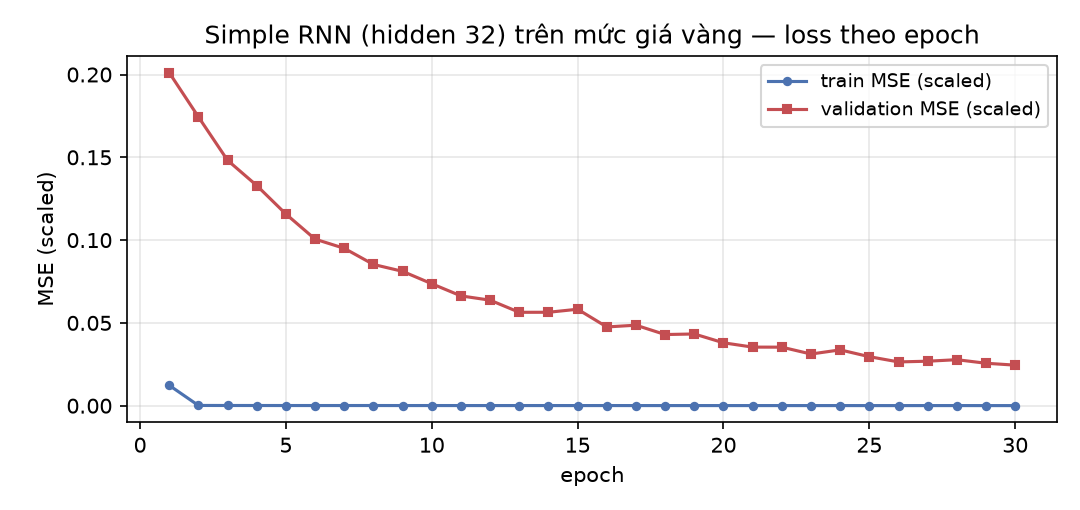
\includegraphics[width=\linewidth]{images/rnn_training_loss.png}
\vspace{0.08cm}
\begin{exampleblock}{\textbf{Đọc đồ thị loss}}
Train loss gần 0; validation loss giảm mạnh rồi ổn định ở mức thấp. Đây là MSE trên dữ liệu đã scale, nên vẫn phải đánh giá sai số trên giá gốc và so với baseline.
\end{exampleblock}
\end{column}
\end{columns}
\end{frame}

% ---------------- SLIDE 37 ----------------
\begin{frame}{Dự báo và phần dư trên tập test}
\centering
\vspace{-0.12cm}
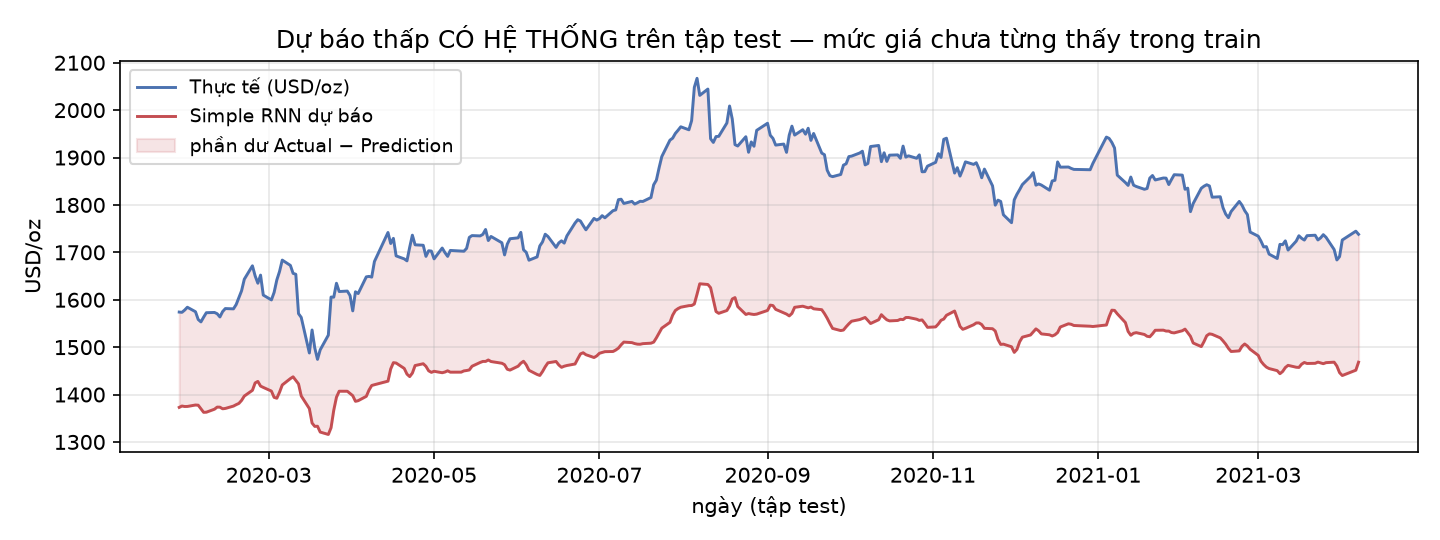
\includegraphics[width=0.80\textwidth,height=3.00cm,keepaspectratio]{images/rnn_actual_vs_pred.png}\\[-0.04cm]
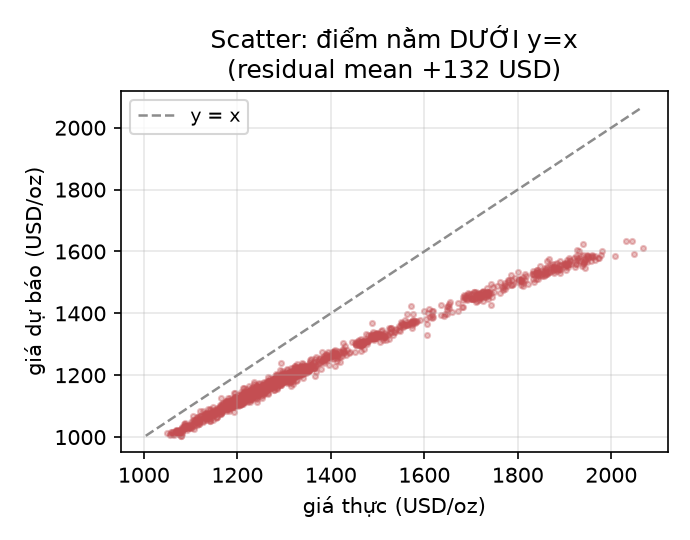
\includegraphics[width=0.80\textwidth,height=3.00cm,keepaspectratio]{images/rnn_residual_scatter.png}
\end{frame}

% ---------------- SLIDE 38 ----------------
\begin{frame}{Đọc kết quả: RNN chưa vượt baseline}
\small
\begin{block}{\textbf{Metrics trên tập test (theo notebook)}}
\centering
\begin{tabular}{lrrrr}
\toprule
\textbf{Mô hình} & \textbf{MAE} & \textbf{RMSE} & \textbf{MAPE} & \textbf{Direction} \\
\midrule
Persistence & 9.2163 & 13.4675 & 0.6714\% & 77.3273\% \\
Simple RNN & 236.1134 & 252.1612 & 16.9713\% & 49.1992\% \\
\bottomrule
\end{tabular}
\end{block}
\vspace{0.12cm}
\begin{columns}[T]
\begin{column}{0.48\textwidth}
\begin{alertblock}{\textbf{Dịch chuyển phân phối}}
Train max: \textbf{850.00}; test min: \textbf{1,049.40}.\\[1mm]
\textbf{100\% giá test vượt train max.}
\end{alertblock}
\end{column}
\begin{column}{0.48\textwidth}
\begin{exampleblock}{\textbf{Dấu hiệu trên biểu đồ}}
Persistence bám sát giá thực. RNN dự báo thấp có hệ thống: phần dư \emph{Actual -- Prediction} dương; điểm phân tán nằm dưới đường $y=x$.
\end{exampleblock}
\end{column}
\end{columns}
\vspace{0.1cm}
\begin{block}{\textbf{Hướng cải thiện}}
Thử dự báo log-return thay cho mức giá, huấn luyện bằng cửa sổ gần thời điểm test hoặc thử GRU/LSTM; luôn so sánh lại với Persistence trên tập test theo đúng thứ tự thời gian.
\end{block}
\end{frame}

\end{document}
